% ------------------------------------------------------------------------
%
% -------------------      Plantilla_UIS.tex       -----------------------
%
% ------------------------------------------------------------------------
% ------------------------------------------------------------------------
% ------------------------------------------------------------------------
% Versión de plantilla para realización de informes de trabajo de grado
% construida para uso de la Universidad Industrial de Santander.
%
% Reservados todos los derechos
%
% Bucaramanga, Colombia
%
% Febrero 03 de 2019
%
% ------------------------------------------------------------------------
% ------------------------------------------------------------------------
% ------------------------------------------------------------------------
%
% --------------------------\documentclass[letter,oneside,12pt,spanish]{report}

\documentclass[letter,oneside,12pt,spanish]{report}
% ------------------------------------------------------------------------
\usepackage{uislatexstyleAPA} % Libreria UIS APA
% ------------------------------------------------------------------------

% --- AQUÍ VAN TODOS LOS PAQUETES --- %
\usepackage[utf8]{inputenc}
\usepackage{epsfig}
\usepackage{amsmath}
\usepackage{amssymb}
\usepackage{graphicx}
\usepackage{float}
\usepackage{multirow}
\usepackage{wrapfig}
\usepackage{enumitem}
\usepackage{xcolor}
\usepackage{caption}
\usepackage{tcolorbox}
\usepackage{subfigure}
\usepackage{listings}
\usepackage{minted}
\usepackage{csquotes}
\usepackage[style=apa]{biblatex}
\usepackage{geometry}
\usepackage{hyperref}
\usepackage{pdfpages}

% --- CONFIGURACIONES DE COLORES --- %
\definecolor{bg}{rgb}{0.95,0.95,0.92}
\definecolor{purple}{rgb}{0.5,0,0.5}
\definecolor{orange}{rgb}{0.9,0.4,0}
\definecolor{codeborder}{RGB}{0,0,0}
\definecolor{codebackground}{RGB}{255,255,255}
\definecolor{codegray}{RGB}{128,128,128}
\definecolor{codegreen}{RGB}{0,153,0}
\definecolor{codeorange}{RGB}{255,125,80}

% --- CONFIGURACIÓN DE LISTINGS --- %
\lstdefinestyle{mystyle}{
	frame=shadowbox,
	backgroundcolor=\color{codebackground},
	commentstyle=\color{codegray},
	keywordstyle=\color{codeorange},
	numberstyle=\tiny\color{codegray},
	stringstyle=\color{codegreen},
	basicstyle=\ttfamily\footnotesize,
	breakatwhitespace=false,
	breaklines=true,
	captionpos=b,
	keepspaces=true,
	numbers=none,
	showspaces=false,
	showstringspaces=false,
	showtabs=false,
	tabsize=2,
	frame=single,
	rulecolor=\color{codeborder},
	framesep=4pt,
	xleftmargin=10pt,
	xrightmargin=10pt,
}
\lstset{style=mystyle}

% --- OTRAS CONFIGURACIONES --- %
\addbibresource{biblio.bib}
\geometry{headheight=15.13202pt}
\captionsetup[figure]{labelfont={bf}, singlelinecheck=false}
\parskip=12pt

\begin{document}                              % Inicio de documento
% ------------------------------------------------------------------------
% Definición silábica de palabras
% ------------------------------------------------------------------------
% \hyphenation{pro-por-cio-nal di-se-ño}
\hypersetup {pdfborder = {0 0 0}}
% ------------------------------------------------------------------------
% Titulo resumido del trabajo que aparecerá en cornisa
% ------------------------------------------------------------------------
\title{AMBIENTE DE APRENDIZAJE PARA LA ENSEÑANZA DE ESTADÍSTICA II}
% ------------------------------------------------------------------------
% Elementos previos al contenido del trabajo
% ------------------------------------------------------------------------ 

\begin{center}

Ambiente de aprendizaje para la enseñanza de Estadística II: un enfoque en teoría, prácticas y autoevaluación\vspace{1.5cm}

Jorge Eduardo Suárez Cortés\\
Daniel Alejandro Sánchez Rodríguez \\ \vspace{1.5cm}

Trabajo de Grado para optar al título de Ingeniero de Sistemas\\ \vspace{1.5cm}

Director\\
Andrés Leonardo González Gómez\\
PhD (c). Ciencias de la Computación\vspace{1.5cm}


Universidad Industrial de Santander\\
Facultad de Ingenierías Fisicomecánicas\\
Escuela de Ingeniería de Sistemas e Informática\\
Ingeniería de Sistemas\\
Bucaramanga\\
2025\\

\end{center}

% Portadilla

\parskip=0pt

\newpage

\titlecontents{paragraph}[0em]{\normalfont\normalsize}{\thecontentslabel. }{}{\titlerule*[1em]{}\contentspage}



\parskip=12pt
\tableofcontents                    

% Tabla de contenido
% ------------------------------------------------------------------------
\newpage

\listoffigures                         % Lista de figuras, tablas y anexos
\newpage
\listoftables
%\listofanexo
% ------------------------------------------------------------------------
\newpage

\chapter*{Glosario}

\begin{description}

\item \textbf{Ambiente Virtual de Aprendizaje (AVA)}: Entorno digital que integra recursos, actividades y herramientas interactivas para apoyar los procesos de enseñanza y aprendizaje en línea o semipresenciales.
\item \textbf{Autoevaluación}: Estrategia pedagógica que permite a los estudiantes valorar su propio proceso de aprendizaje mediante actividades de retroalimentación automática.
\item \textbf{Base de Datos}: Conjunto estructurado de información almacenada de manera organizada que permite el acceso, la gestión y la actualización de datos académicos y de evaluación.
\item \textbf{Docker}: Plataforma de virtualización ligera que permite empaquetar aplicaciones y servicios en contenedores portables, facilitando su despliegue en diferentes entornos.
\item \textbf{Estadística Inferencial}: Rama de la estadística que utiliza datos muestrales para realizar inferencias, estimaciones o pruebas sobre parámetros poblacionales.
\item \textbf{Google Colab}: Herramienta en la nube que permite ejecutar código en Python y R desde un navegador, facilitando la realización de prácticas y análisis de datos sin necesidad de instalación local.
\item \textbf{Grader}: Sistema automatizado de evaluación que corrige ejercicios prácticos, especialmente de programación y estadística, generando resultados inmediatos.
\item \textbf{LMS (Learning Management System)}: Sistema de gestión del aprendizaje que permite planificar, implementar y evaluar procesos educativos en entornos virtuales. Facilita la creación de cursos, administración de contenidos, seguimiento del progreso de los estudiantes y la comunicación entre docentes y alumnos.
\item \textbf{Moodle}: Plataforma de gestión de aprendizaje (LMS, por sus siglas en inglés) de código abierto, utilizada para crear cursos en línea, administrar contenidos y facilitar la comunicación entre docentes y estudiantes.
\item \textbf{Node.js}: Entorno de ejecución de JavaScript orientado al desarrollo de aplicaciones web y servidores, utilizado para gestionar la comunicación entre sistemas del entorno virtual.
\item \textbf{Playit.gg}: Servicio que permite crear túneles seguros para acceder a aplicaciones locales desde internet, sin necesidad de configuraciones avanzadas en redes.

\end{description}


% ------------------------------------------------------------------------
\newpage

% Contenido del Informe
% ------------------------------------------------------------------------
\newpage

\chapter*{Resumen}

\footnotesize{
\begin{description}
  \item[Título:] Ambiente de aprendizaje para la enseñanza de Estadística II: un enfoque en teoría, prácticas y autoevaluación.
  \astfootnote{Trabajo de grado}
  \item[Autores:] Jorge Eduardo Suárez Cortés y Daniel Alejandro Sánchez Rodríguez.
  \asttfootnote{Facultad de Ingenierías Fisicomecánicas. Escuela de Ingeniería de Sistemas e Informática.\\
  	Director: Andrés Leonardo Gonzáles Gómez}
  \item[Palabras Clave:]Ambiente virtual de aprendizaje, Moodle, Estadística II, Autoevaluación.
  \item[Descripción:] El presente trabajo de grado describe el diseño, desarrollo e implementación 
  de un ambiente de aprendizaje virtual para la asignatura Estadística II, dirigida a estudiantes de 
  la Escuela de Ingeniería de Sistemas e Informática de la Universidad Industrial de Santander. El 
  ambiente fue construido sobre la plataforma Moodle, con el objetivo de ofrecer una experiencia de 
  aprendizaje más activa, significativa y continua mediante la integración sistemática de contenidos 
  teóricos, ejercicios prácticos y mecanismos de evaluación formativa, tales como autoevaluaciones y 
  retroalimentación inmediata.

  El enfoque pedagógico del entorno se basa en el aprendizaje activo y la construcción progresiva del 
  conocimiento, promoviendo la participación continua del estudiante y el desarrollo de competencias 
  relacionadas con el análisis estadístico y la interpretación de datos. Las actividades propuestas están 
  diseñadas para favorecer la autonomía del aprendizaje. Los resultados obtenidos sugieren que el uso del
  ambiente virtual contribuye a mejorar la comprensión de los contenidos estadísticos, así como a incrementar 
  la motivación y el compromiso de los estudiantes con su proceso de formación. Esta propuesta representa 
  una alternativa metodológica y tecnológica que responde a las necesidades actuales de la educación superior
  en el ámbito de la ingeniería de sistemas, especialmente en contextos donde la articulación entre teoría y 
  práctica resulta esencial para el desarrollo de competencias profesionales.
  
  
\end{description}}\normalsize

% ------------------------------------------------------------------------

\newpage

\chapter*{Abstract}

\footnotesize{
\begin{description}
  \item[Title:] Learning Environment for the Teaching of Statistics II: A Focus on Theory, Practice, and Self-Assessment.
  \astfootnote{Degree Work}
  \item[Authors:] Jorge Eduardo Suárez Cortés y Daniel Alejandro Sánchez Rodríguez.
  \asttfootnote{Faculty of Physicomechanical Engineering. School of Systems and Computer Engineering.\\
  	Director: Andrés Leonardo Gonzáles Gómez}
  \item[Key words:] Virtual learning environment, Moodle, Statistics II, Self-assessment.
  \item[Description:]This thesis describes the design, development, and implementation 
  of a virtual learning environment for the Statistics II course, aimed at students of 
  the School of Systems Engineering and Computer Science at the Industrial University of Santander. The 
  environment was built on the Moodle platform, with the aim of offering a more active, meaningful, and 
  continuous learning experience through the systematic integration of theoretical content, practical 
  exercises, and formative assessment mechanisms, such as self-assessments and immediate feedback.

  The pedagogical approach of the environment is based on active learning and the progressive construction of 
  knowledge, promoting continuous student participation and the development of skills 
  related to statistical analysis and data interpretation. The proposed activities are 
  designed to encourage autonomous learning. The results obtained suggest that the use of the
  virtual environment contributes to improving the understanding of statistical content, as well as increasing 
  student motivation and commitment to their training process. This proposal represents 
  a methodological and technological alternative that responds to the current needs of higher education
  in the field of systems engineering, especially in contexts where the articulation between theory and 
  practice is essential for the development of professional skills.

\end{description}}\normalsize

% Abstract

% ------------------------------------------------------------------------
% Capítulos
% ------------------------------------------------------------------------
\newpage

\nnchapter{Introducción}



% ------------------------------------------------------------------------

\newpage


\chapter{Objetivos}

\section{Objetivo General}

\begin{itemize}
    \item Diseñar y desarrollar un entorno virtual para la asignatura de Estadística II, de la Escuela de Ingeniería de Sistemas e 
    Informática de la UIS, que facilite la ejecución de un plan de aula propuesto para la práctica, el aprendizaje y la autoevaluación 
    del contenido de la asignatura, mediante herramientas de Python y R.
\end{itemize}

\section{Objetivos Especificos}

\begin{itemize}
    \item Diseñar un plan de aula modular para la asignatura Estadística II que organice los contenidos teóricos y prácticos en 
    unidades interactivas basadas en Colab Notebooks, Python y R, e incluya calificadores automáticos y ejercicios con retroalimentación 
    instantánea.
    
    \item Implementar un ambiente de aprendizaje virtual en la plataforma Moodle que integre las tecnologías definidas (Colab Notebooks, 
    Python y R) y organice los contenidos teóricos y prácticos junto con materiales didácticos de apoyo, consolidando una experiencia 
    formativa práctica y accesible para la asignatura Estadística II.
    
    \item Establecer instrumentos de medición para las actividades prácticas y autoevaluativas en Moodle (desarrolladas con Python y R), 
    que permitan medir el logro de los resultados de aprendizaje durante el desarrollo del proyecto en el curso de Estadística II.

    \item Pilotear el ambiente virtual de aprendizaje diseñado, con sus contenidos interactivos e instrumentos de evaluación, en por lo 
    menos dos grupos de Estadística II de la Escuela de Ingeniería de Sistemas e Informática de la UIS, con el fin de validar su 
    usabilidad, satisfacción y efectividad en el logro de los resultados de aprendizaje.

\end{itemize}

% ------------------------------------------------------------------------

\newpage

\chapter{Marco Teorico}

\section{Estadística}

La estadística constituye una herramienta fundamental en la ciencia, la ingeniería y la administración, al proporcionar métodos rigurosos para recopilar, organizar, presentar, analizar e interpretar datos con el fin de apoyar la toma de decisiones. En la actualidad, desempeña un papel crucial en el análisis de sistemas complejos, la mejora de procesos y el control de calidad en distintos entornos académicos, industriales y científicos.

De acuerdo con \textcite{montgomery1996}, la estadística moderna se divide en dos grandes áreas: estadística descriptiva y estadística inferencial. La primera se ocupa de técnicas que permiten resumir y describir de manera gráfica o numérica los datos disponibles, mientras que la segunda se orienta hacia la formulación de generalizaciones o la toma de decisiones sobre una población a partir de la información contenida en una muestra.

En el contexto de este proyecto, la atención se centra en la estadística inferencial, dado que la asignatura Estadística II aborda conceptos como la estimación puntual, la construcción de intervalos de confianza, las pruebas de hipótesis y el estudio de distribuciones muestrales. Dichos contenidos resultan esenciales para obtener conclusiones válidas a partir de datos incompletos o parciales. Al tratarse de una asignatura que combina teoría matemática con aplicaciones prácticas en problemas reales, se requiere no solo comprender los fundamentos conceptuales, sino también desarrollar competencias aplicadas. Por ello, este proyecto plantea el diseño de un entorno virtual interactivo que permita a los estudiantes ejercitar dichos conceptos con datos reales, actividades prácticas y retroalimentación inmediata.

\subsection{Estadística Inferencial}

La estadística inferencial es considerada una de las ramas más potentes y aplicadas de la disciplina. Su propósito central es extraer conclusiones sobre una población a partir de la información proporcionada por una muestra. Según \textcite{montgomery1996}, la mayoría de las aplicaciones estadísticas en ciencia, ingeniería y administración incorporan procedimientos de inferencia y toma de decisiones.

Entre los conceptos más relevantes que sustentan esta disciplina se encuentran:

\begin{itemize}
	\item \textbf{Distribuciones muestrales}: distribuciones de probabilidad de estadísticas como la media, la proporción o la varianza, que permiten describir la variabilidad esperada de los estimadores a partir de distintas muestras.
	
	\item \textbf{Estimación de parámetros}: procedimientos mediante los cuales se obtienen valores aproximados de parámetros poblacionales utilizando la información muestral.
	
	\item \textbf{Pruebas de hipótesis}: métodos formales que permiten aceptar o rechazar proposiciones acerca de parámetros poblacionales, basándose en la evidencia empírica extraída de una muestra.
\end{itemize}

\section{Ambientes de aprendizaje}

\subsection{Políticas TIC en educación}

El diseño de ambientes de aprendizaje en la educación superior no solo responde a fundamentos pedagógicos y tecnológicos, sino también a marcos normativos e institucionales que orientan su desarrollo. En este sentido, la Política Institucional de Tecnologías de la Información y la Comunicación (TIC) de la Universidad Industrial de Santander, establecida mediante el Acuerdo del Consejo Superior No. 051 de 2009, constituye un referente clave para la integración de recursos digitales en los procesos académicos.

Dicha política busca garantizar el acceso equitativo a la información, fomentar la innovación pedagógica y promover la incorporación de tecnologías abiertas e interoperables en la formación universitaria. Asimismo, establece como principios fundamentales el fortalecimiento de los procesos de enseñanza-aprendizaje, la inclusión de toda la comunidad académica en el uso de las TIC y la consolidación de una cultura institucional que aproveche estas herramientas para el mejoramiento continuo de la calidad educativa \parencite{uis2009}.

De esta forma, el presente proyecto se enmarca en los lineamientos de la Política TIC, ya que aprovecha plataformas como Moodle y Google Colab para potenciar la enseñanza de la estadística mediante recursos digitales interactivos, autoevaluaciones y retroalimentación automática. Esto permite articular los objetivos pedagógicos con los principios institucionales de innovación, inclusión y acceso abierto al conocimiento.

\subsection{Ambiente de aprendizaje}

El concepto de ambiente de aprendizaje se refiere al conjunto de condiciones, espacios, interacciones y recursos que permiten y favorecen el desarrollo de procesos educativos efectivos. Este término alude a un escenario dinámico en el que los individuos desarrollan capacidades, competencias, habilidades y valores. Es decir, no se trata de un espacio fijo ni neutral, sino de un entorno que debe transformarse en función de las necesidades de los estudiantes y de las innovaciones educativas \parencite{castro2019}.

En este sentido, un ambiente de aprendizaje no se limita al aula física, sino que constituye una construcción pedagógica en la que intervienen aspectos sociales, culturales, tecnológicos y metodológicos. De acuerdo con \textcite{castro2019}, un ambiente de aprendizaje debe ser:

\begin{itemize}
	\item Flexible y adaptable a diferentes contextos y tecnologías.
	\item Fomentar la interacción social y la construcción colectiva del conocimiento.
	\item Proporcionar recursos adecuados, incluidos los tecnológicos, que potencien las competencias estudiantiles.
	\item Promover el rol activo del docente como diseñador, facilitador y mediador del aprendizaje.
\end{itemize}

Desde esta perspectiva, los ambientes de aprendizaje se conciben como espacios dinámicos e integrales, que van más allá de la transmisión de información y buscan estimular la participación activa, la autonomía y la construcción colaborativa del conocimiento.

\subsection{Ambientes virtuales de aprendizaje}

El avance de las tecnologías digitales ha posibilitado la transición de los entornos tradicionales hacia los Ambientes Virtuales de Aprendizaje (AVA). Estos se definen como plataformas tecnológicas que integran recursos didácticos, actividades de aprendizaje, espacios de interacción y mecanismos de evaluación para facilitar procesos formativos en entornos digitales \parencite{salinas2004}.

En coherencia con las características planteadas por \textcite{castro2019}, los AVA son flexibles y adaptables a diferentes contextos, fomentan la interacción social y colaborativa, proporcionan recursos tecnológicos que amplían las competencias estudiantiles y posicionan al docente como un mediador y facilitador del aprendizaje.

Uno de los sistemas más representativos en este campo es Moodle, un Learning Management System (LMS) de código abierto que ha sido adoptado globalmente en educación superior debido a su enfoque pedagógico constructivista, su escalabilidad y su facilidad de integración con otras herramientas \parencite{dougiamas2003}. Moodle permite gestionar cursos, estudiantes, actividades y evaluaciones, convirtiéndose en un eje articulador del proceso formativo.

En el contexto del presente proyecto, Moodle constituye el espacio institucional de referencia en la UIS, donde los estudiantes acceden a materiales de teoría, actividades interactivas y prácticas en Google Colab, además de las autoevaluaciones conectadas con el backend. Su importancia radica en que integra de manera armónica la teoría, la práctica y la retroalimentación automática, consolidando un entorno virtual de aprendizaje efectivo.



\section{Tecnologías implementadas en el proyecto}

\subsection{Node.js y Express.js}

Node.js es un entorno de ejecución basado en el motor V8 de Google Chrome que permite ejecutar JavaScript en el lado del servidor, diseñado bajo un modelo de I/O no bloqueante. Esto lo convierte en una herramienta adecuada para aplicaciones que requieren manejar múltiples solicitudes concurrentes, como plataformas de aprendizaje en línea \parencite{tilkov2010}.

Express.js es un framework minimalista para Node.js que facilita la construcción de APIs y aplicaciones web mediante la organización de rutas, middleware y controladores \parencite{brown2019}. En el proyecto, Node.js y Express.js cumplen el rol de backend principal, gestionando la validación de respuestas de estudiantes, el control de intentos y la comunicación con la base de datos MariaDB.

\subsection{React.js}

React.js es una biblioteca de JavaScript desarrollada por Facebook que permite construir interfaces de usuario basadas en componentes reutilizables \parencite{banks2017}. Su arquitectura con virtual DOM optimiza la actualización de vistas, mejorando la eficiencia y la experiencia de usuario.

El frontend, desarrollado en React.js, centraliza la gestión de calificaciones y el control de intentos de los estudiantes. Su principal ventaja es la transparencia: ante cualquier discrepancia con la calificación calculada por el backend (Node.js), un instructor puede revisar tanto el código enviado por el estudiante como la nota obtenida. Esto facilita una verificación rápida y fundamentada, garantizando la equidad en la evaluación.

\subsection{Bases de datos relacionales (MariaDB)}

MariaDB es un sistema de gestión de bases de datos relacional de código abierto, derivado de MySQL, que organiza los datos en tablas relacionadas bajo el modelo relacional propuesto por \textcite{codd1970}.

Su función en el proyecto es ser el repositorio central de información, donde se almacenan los registros de estudiantes, intentos de ejercicios, calificaciones y respuestas. Gracias a sus características de integridad y consistencia, MariaDB asegura la fiabilidad en el almacenamiento de los resultados generados en los procesos de autoevaluación.

\subsection{Virtualización y contenedores (Docker)}

Docker es una plataforma de contenedores ligeros que empaqueta aplicaciones y dependencias en un entorno aislado, lo que garantiza portabilidad y reproducibilidad \parencite{merkel2014}.

En el proyecto, Docker permite desplegar servicios como el backend, frontend, playit.gg y la base de datos en un entorno controlado, asegurando que las pruebas piloto y los despliegues sean consistentes sin importar el sistema operativo. Su uso facilita la escalabilidad y reduce los problemas de compatibilidad entre entornos de desarrollo y producción.

\subsection{Moodle como LMS}

Moodle es un sistema de gestión de aprendizaje (LMS) de código abierto ampliamente utilizado en la educación superior. Ofrece herramientas para gestionar cursos, usuarios, recursos y actividades de evaluación \parencite{dougiamas2003}.

En este proyecto, Moodle funciona como el entorno de acceso institucional provisto por la UIS, donde los estudiantes encuentran los enlaces a los notebooks de Google Colab, las actividades prácticas y los recursos teóricos. Moodle sirve como el punto de integración pedagógica que articula los recursos tecnológicos desarrollados.

\subsection{Python y R}

Python y R son lenguajes de programación consolidados en el campo del análisis estadístico y la ciencia de datos. Python, gracias a bibliotecas como NumPy, SciPy y Pandas, se ha convertido en una herramienta versátil para la enseñanza y aplicación de métodos estadísticos \parencite{mckinney2017}. R, por su parte, es un lenguaje especializado en estadística y visualización de datos, ampliamente usado en contextos académicos \parencite{rcoreteam2023}.

En el proyecto, para el desarrollo de los graders se emplearán ambos lenguajes de programación, lo que permitirá dotarlos de una mayor versatilidad en su uso.

\subsection{Google Colab}

Google Colab es una plataforma en la nube que permite ejecutar notebooks de Python sin necesidad de instalar software localmente. Combina teoría, código ejecutable y resultados en un único entorno interactivo \parencite{bisong2019}.

Su integración en el proyecto permite a los estudiantes resolver ejercicios en tiempo real, ejecutar simulaciones y enviar sus respuestas al backend para validación. Además, Colab facilita el aprendizaje activo y autónomo.

\subsection{Graders y autoevaluación automatizada}

Los graders son sistemas de evaluación automática que comparan respuestas de estudiantes con soluciones esperadas, otorgando calificaciones y retroalimentación inmediata \parencite{kurnia2001}. Herramientas como nbgrader o Otter-Grader han demostrado su efectividad en la enseñanza de programación y estadística.

En este proyecto, los graders están implementados en el backend desarrollado con Node.js y conectados a los notebooks de Colab. De esta forma, los estudiantes reciben retroalimentación instantánea, lo que fomenta el aprendizaje autónomo y reduce la carga de corrección manual para los docentes.

\subsection{Playit.gg y tunelización de servicios}

Playit.gg es una herramienta que permite crear túneles seguros entre una máquina local y la web pública, facilitando la exposición de servicios locales sin necesidad de configuración compleja de red.

Durante el desarrollo y pruebas piloto del proyecto, Playit.gg se utiliza para exponer el backend y el frontend alojados en contenedores Docker hacia los estudiantes y notebooks de Colab. Esta estrategia permite realizar pilotos de manera controlada.


% ------------------------------------------------------------------------
\newpage


\chapter{Estado del Arte}

\section{Introducción}
La enseñanza de la estadística en educación superior presenta desafíos significativos debido a la abstracción de sus conceptos y la necesidad de aplicar teoría a problemas del mundo real. En este contexto, los Ambientes Virtuales de Aprendizaje (AVA) y plataformas digitales han emergido como recursos clave para mediar procesos formativos, permitiendo integrar materiales, actividades prácticas y evaluaciones \parencite{AlHaddad2024}. Sin embargo, aunque las soluciones existentes han avanzado en accesibilidad y organización de contenidos, persisten limitaciones relacionadas con la retroalimentación inmediata, la integración de entornos de análisis de datos y la evaluación automatizada de procesos complejos como la estadística inferencial.

\section{Antecedentes}

\subsection{La evolución de los LMS}
Los sistemas de enseñanza asistida han experimentado una evolución significativa desde sus orígenes en la década de 1960 hasta la consolidación de plataformas como Moodle en la actualidad. Uno de los primeros hitos fue el desarrollo de \textit{PLATO} (Programmed Logic for Automated Teaching Operations) en la Universidad de Illinois en 1960. Este sistema permitía la entrega de contenidos programados, evaluaciones automatizadas, comunicación entre estudiantes y docentes mediante foros y mensajería, además de seguimiento del progreso individual. A pesar de los altos costos por el uso de mainframes, PLATO fue implementado en más de 1.000 instituciones educativas y sentó las bases técnicas y pedagógicas de los actuales LMS \parencite{Woolley2016}.

En 1965, Patrick Suppes y Richard Atkinson, en la Universidad de Stanford, exploraron el uso de computadoras para la enseñanza de matemáticas y lectura en escuelas de Palo Alto. Su sistema ofrecía retroalimentación inmediata y ramificaciones condicionales según el desempeño del estudiante. Los resultados mostraron una mejora del 25\% en la retención de conceptos matemáticos básicos en comparación con métodos tradicionales, lo que evidenció el potencial del aprendizaje asistido por computadora para personalizar la enseñanza \parencite{Suppes1966}.

Posteriormente, entre 1973 y 1977, el \textit{National Development Programme in Computer Aided Learning} (NDPCAL) en el Reino Unido financió más de 30 proyectos universitarios que integraban gestión de contenidos digitales, evaluación automatizada y seguimiento del progreso estudiantil. Uno de los proyectos más destacados fue implementado en la Universidad de Leeds, donde se logró reducir el tiempo de retroalimentación en cursos de estadística de semanas a horas, mejorando significativamente la experiencia de aprendizaje \parencite{Hooper1977}.

El punto de inflexión en la historia de los LMS modernos llegó el 20 de agosto de 2002, cuando Martin Dougiamas publicó la primera versión estable de Moodle 1.0. Desarrollado como parte de su tesis doctoral en la Universidad de Curtin (Australia), Moodle fue concebido bajo principios constructivistas y liberado como software de código abierto. Esta primera versión permitía la creación de cursos interactivos, gestión de tareas, foros de discusión y evaluaciones básicas. A pesar de su simplicidad inicial, Moodle fue rápidamente adoptado por comunidades educativas de todo el mundo, traducido a múltiples idiomas y adaptado a diversos contextos pedagógicos \parencite{Moodle2024}.

Hoy en día, Moodle supera los 160.000 sitios registrados y 240 millones de usuarios en más de 240 idiomas. Es utilizado por aproximadamente el 67\% de las instituciones de educación superior a nivel mundial. Su arquitectura abierta y modular permite integrar herramientas especializadas como Jupyter Notebook, nbgrader, R, Python y entornos de evaluación automática, lo que lo ha convertido en una plataforma clave para la enseñanza de la estadística y la ciencia de datos en la educación superior \parencite{Goh2025, Moodle2024}.

La Figura~\ref{fig:LineaTiempo} muestra la línea de tiempo de la evolución de los LMS, destacando los hitos más importantes que llevaron a su consolidación.

\begin{figure}[ht]
	\centering
    \captionof{figure}{ \\ \vspace{0.5cm} Estado del arte. \textbf{Linea de tiempo con base en diversas fuentes históricas.}.}
	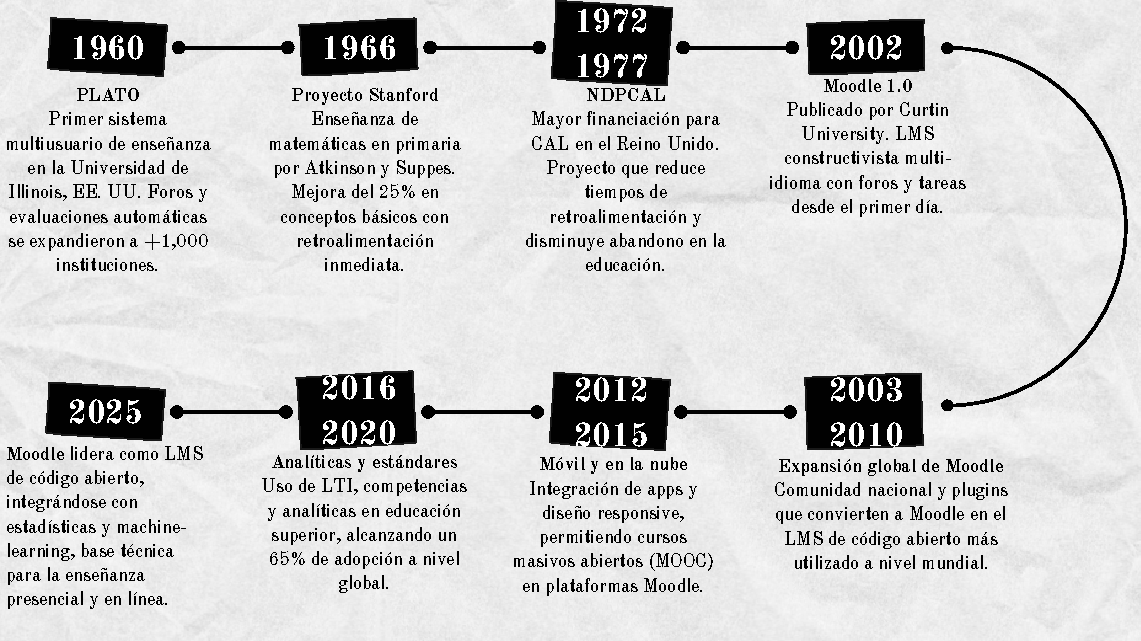
\includegraphics[width=1\textwidth]{Figs/Linea del Tiempo.pdf}
	\label{fig:LineaTiempo}
	\\Fuente: Autores
\end{figure}

\subsection{Plataformas de Aprendizaje}
Las plataformas de gestión del aprendizaje (LMS) como Moodle han revolucionado la educación digital desde su implementación. El caso pionero de la Universidad de Curtin en Australia en 2002 demostró que la adopción de Moodle en cursos de estadística descriptiva resultó en una mejora significativa en la participación estudiantil y una reducción del 30\% en los índices de reprobación, atribuible a la organización modular de contenidos y el acceso asíncrono a materiales \parencite{Pacheco2025}. Este tipo de resultados se alinea con el ciclo de validación continua que suele seguirse en la implementación de un LMS, como se resume en la Figura~\ref{fig:LMS}, donde se observa cómo la revisión iterativa de requisitos, contenidos y pruebas permite alcanzar un entorno de aprendizaje funcional y adaptado al contexto institucional.

\begin{figure}[ht]
    \centering
    \captionof{figure}{ \\ \vspace{0.5cm} Estado del arte. \textbf{Plataformas de aprendizaje}.}
    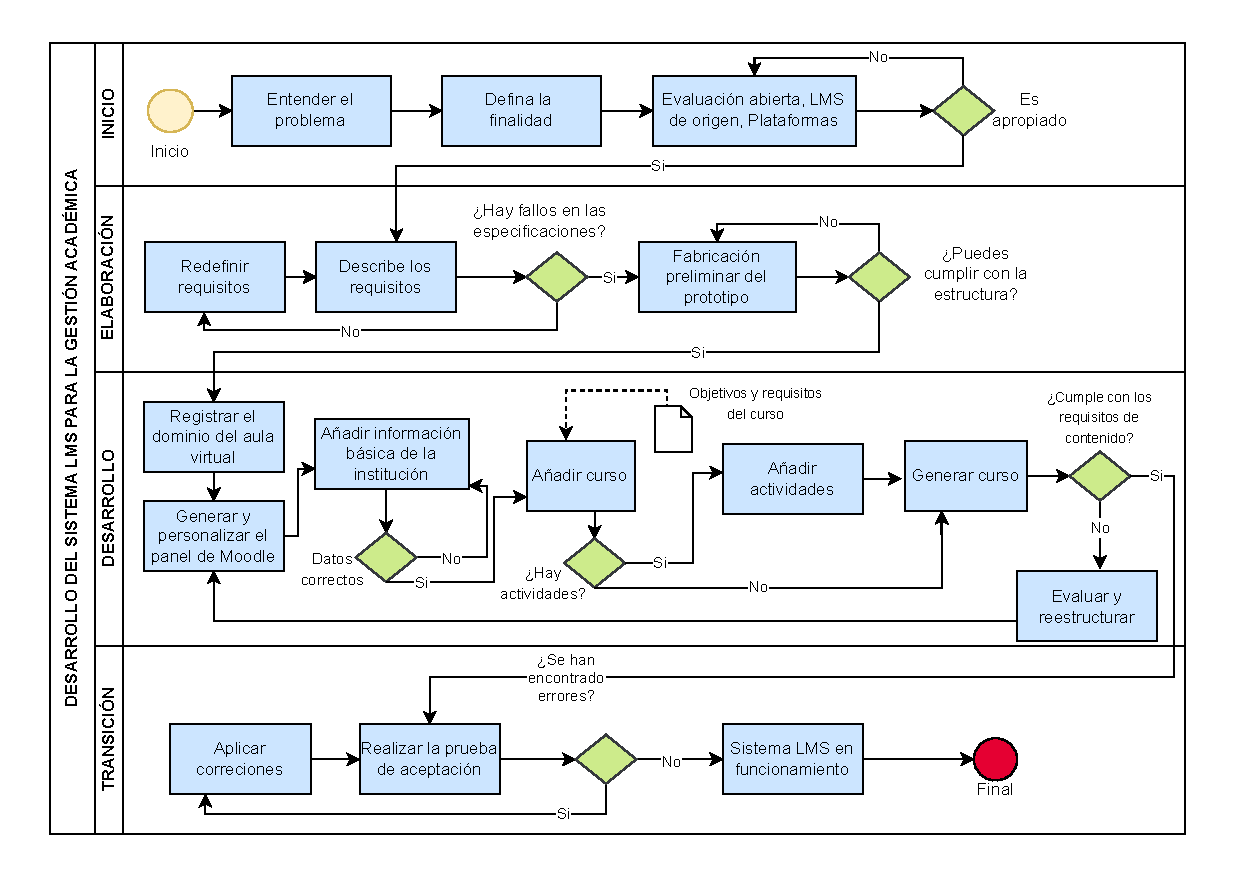
\includegraphics[width=1\textwidth]{Figs/LMS.pdf}
    \label{fig:LMS}
    \\Fuente: Adaptada de \textcite{Pacheco2025}
\end{figure}

Más recientemente, en 2025, la Universidad Nacional de Educación a Distancia (UNED) de España desarrolló un MOOC de estadística en Moodle que alcanzó una tasa de finalización del 68\%, superior al promedio de cursos masivos. Este éxito se atribuyó al uso de evaluaciones automáticas, foros moderados y contenido multimedia adaptativo \parencite{Goh2025}. En contextos de menores recursos, la Universidad Pública de El Alto en Bolivia implementó Moodle para Estadística II en 2024, logrando mejoras significativas en la claridad de contenidos y el rendimiento académico de los estudiantes \parencite{Ndibalema2025}.

Estos ejemplos demuestran que Moodle no solo cumple funciones administrativas, sino que puede ser una fuente valiosa de información para mejorar la enseñanza de la estadística cuando se complementa con herramientas externas de análisis y práctica computacional. Las analíticas de aprendizaje basadas en el uso del LMS se han convertido en un campo emergente, donde la persistencia y constancia de los estudiantes en el uso de la plataforma se correlaciona directamente con el éxito académico, abriendo la puerta a modelos predictivos de intervención temprana \parencite{Goh2025}.

\subsection{Sistemas de Autoevaluación y Retroalimentación Automatizada}
La retroalimentación inmediata es crucial en la consolidación del aprendizaje estadístico. Mientras que los entornos tradicionales se centran en respuestas cerradas, las herramientas modernas han expandido su alcance hacia problemas complejos. El proyecto \textit{nbgrader}, implementado en la Universidad de Berkeley en 2017, permitió evaluar automáticamente tareas de estadística en Jupyter Notebooks, validando tanto la exactitud numérica como la lógica del código en Python, resultando en una reducción del 40\% en el tiempo de calificación y un aumento en la precisión de las evaluaciones \parencite{Blank2017}.

Sin embargo, investigaciones recientes identifican limitaciones persistentes. En 2024, la Universidad de Kuwait implementó un sistema de autoevaluación en estadística inferencial que, aunque efectivo para respuestas numéricas, no pudo evaluar el razonamiento estadístico ni la justificación de procedimientos, evidenciando la necesidad de graders más avanzados que trasciendan la simple comparación de valores \parencite{AlHaddad2024}.

Estas limitaciones subrayan la importancia de desarrollar sistemas de evaluación más sofisticados. Diversos estudios han sugerido que una alternativa futura es integrar graders más avanzados que almacenen y auditen código, permitiendo no solo verificar respuestas correctas o incorrectas, sino también analizar el proceso de resolución seguido por el estudiante, aumentando la transparencia y equidad en la evaluación.


\subsection{Arquitectura tecnológica para la educación}

En el ámbito de la enseñanza de la estadística, la discusión sobre arquitecturas tecnológicas ha pasado de enfocarse en plataformas de gestión administrativa hacia propuestas que buscan integrar entornos de análisis, retroalimentación inmediata y evaluación automatizada como se puede ver presente en la Figura~\ref{fig:architecture_E-learning}. Moodle continúa siendo una referencia obligada en la educación digital, especialmente por su capacidad para organizar contenidos y actividades. Sin embargo, varios estudios coinciden en que, aunque resulta eficaz para estructurar cursos, no responde por completo a las exigencias de la enseñanza de la estadística inferencial, en la que interesa no solo el resultado final, sino también el razonamiento seguido por el estudiante \parencite{Pacheco2025, Ndibalema2025}.

\begin{figure}[ht]
    \centering
    \captionof{figure}{ \\ \vspace{0.5cm} Estado del arte. \textbf{Arquitectura tecnológica para la educación}.}
    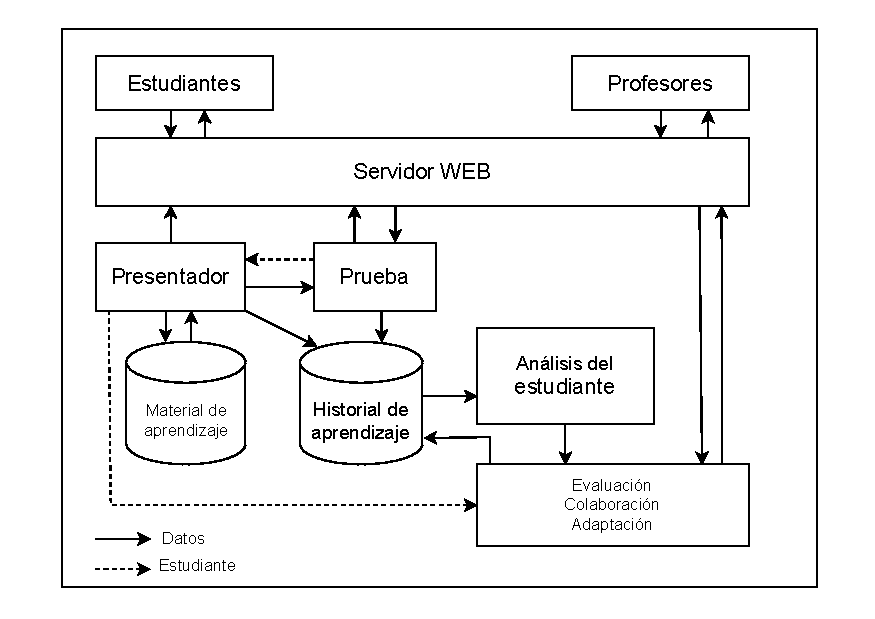
\includegraphics[width=0.9\textwidth]{Figs/Arquitectura_E-learning.pdf}
    \label{fig:architecture_E-learning}
    \\Fuente: Adaptada de \textcite{Mostefai2025}
\end{figure}


Ante esta limitación, algunas instituciones han apostado por combinar los LMS con entornos de programación y análisis de datos. Un ejemplo temprano es JupyterHub con nbgrader, desarrollado en la Universidad de California, Berkeley, que se consolidó como un referente en cursos masivos de ciencia de datos al permitir la entrega, ejecución y calificación automática de notebooks de Python \parencite{berkeley2018}. Por otro lado, la Universidad de Auckland ha incorporado RStudio Cloud para facilitar la práctica con R en cursos de inferencia y análisis de datos, priorizando la accesibilidad en la web \parencite{rubio2023}. Finalmente, en Carnegie Mellon University se ha implementado Autolab, pensado para la calificación de código en línea con control de intentos y reportes de error detallados \parencite{rubio2023}.

El diseño de entornos educativos digitales exige arquitecturas escalables, flexibles y seguras. En 2025, Mostefai propuso una arquitectura de microservicios para plataformas educativas que separa la lógica de negocio, la visualización de resultados y la gestión de datos en componentes independientes se puede ver representado en la Figura~\ref{fig:Microservicios}. Esta arquitectura permitió escalar cursos de estadística con más de 5.000 estudiantes simultáneos sin pérdida de rendimiento, mejorando significativamente la mantenibilidad y escalabilidad de los sistemas \parencite{Mostefai2025}.

\begin{figure}[ht]
    \centering
    \captionof{figure}{ \\ \vspace{0.5cm} Estado del arte. \textbf{Arquitectura de microservicios}.}
    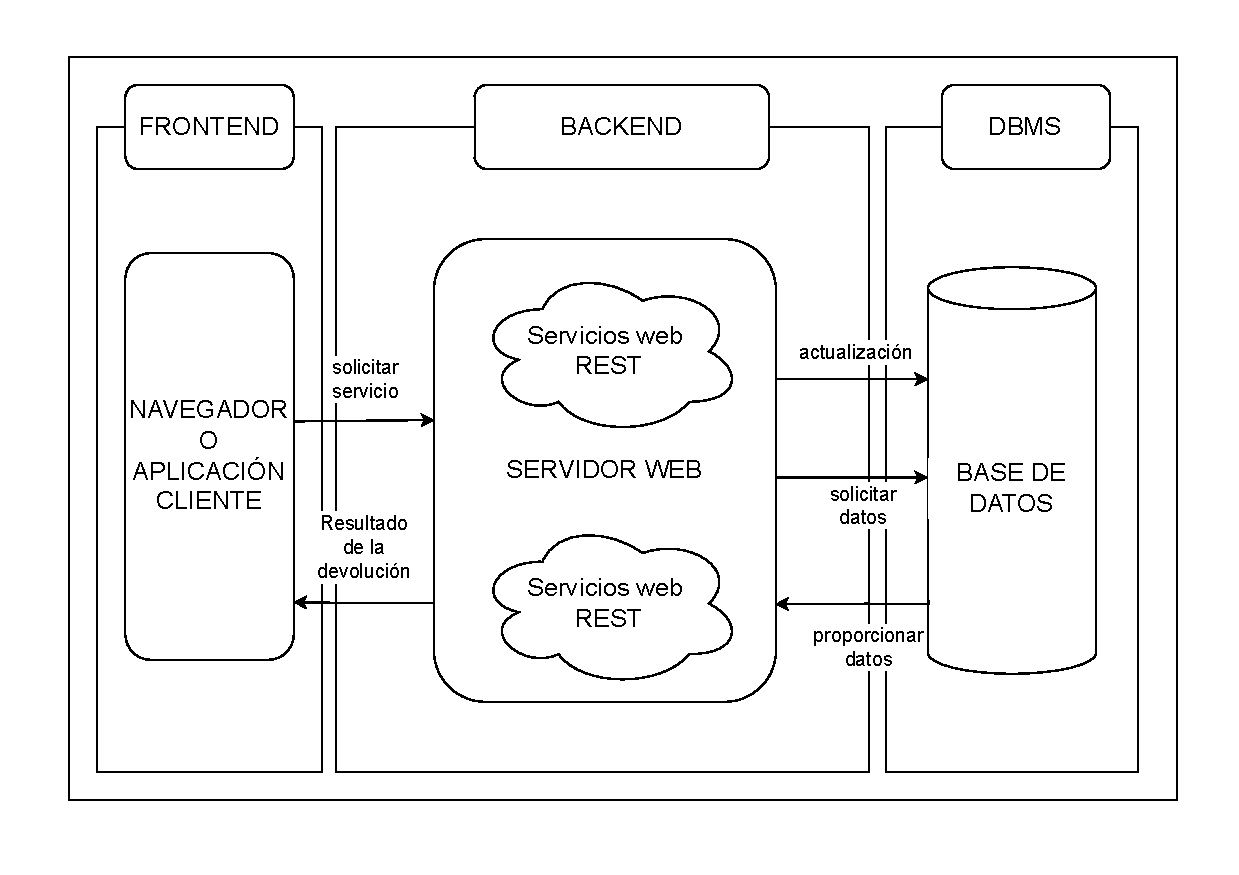
\includegraphics[width=0.9\textwidth]{Figs/Microservicios.pdf}
    \label{fig:Microservicios}
    \\Fuente: Adaptada de \textcite{Mostefai2025}
\end{figure}



Estas experiencias muestran un avance real hacia la automatización de la evaluación y la integración con el aprendizaje activo. Sin embargo, también dejan en evidencia limitaciones importantes. Por un lado, dependen de infraestructura institucional robusta o de licencias de pago, lo que restringe su uso en contextos de menor presupuesto. Además, suelen enfocarse en verificar la exactitud del código o los resultados numéricos, pero no siempre logran capturar la trazabilidad del razonamiento estadístico, que es clave en la formación en inferencia \parencite{alhaddad2024}.



\subsection{Antecedentes nacionales y la UIS}

En el contexto colombiano, la Universidad Industrial de Santander (UIS) ha sido pionera en el 
desarrollo de iniciativas que fortalecen la enseñanza y el aprendizaje de la estadística, 
articulando recursos digitales, programas de formación y unidades de análisis institucional. 
Desde mediados de la década de 2010, el Grupo SIMON de la UIS diseñó el software Evolución, una 
herramienta de modelado y simulación con dinámica de sistemas utilizada como apoyo en procesos 
formativos y de investigación, lo que refleja una apuesta temprana por el uso de simuladores en 
la enseñanza de disciplinas cuantitativas \parencite{simon2016}.

De manera complementaria, la Dirección de Nuevas Tecnologías de la Información y las Comunicaciones
 (NTIC) de la UIS consolidó un repositorio de software y simuladores disponibles para estudiantes 
 y docentes, los cuales abarcan desde áreas de ingeniería hasta aplicaciones estadísticas, 
 contribuyendo al fortalecimiento del aprendizaje autónomo y práctico \parencite{nticsf}. Esta 
 apuesta tecnológica se ha acompañado de la creación de la Unidad de Información y Análisis 
 Estadístico (UIAES), orientada a centralizar datos institucionales y a promover el uso de la 
 estadística como herramienta de apoyo en la gestión académica y administrativa, lo que evidencia
  una integración de la estadística no solo en la docencia, sino también en la toma de decisiones 
  estratégicas \parencite{uiassf}.

En el ámbito de la formación avanzada, la UIS ha ofrecido desde hace más de dos décadas la 
Especialización en Estadística, adscrita a la Escuela de Matemáticas. Este programa de posgrado 
se ha consolidado como referente nacional, orientando profesionales en el manejo de metodologías 
estadísticas aplicadas en contextos empresariales, educativos y de investigación 
\parencite{especializacionstatssf}. Estas iniciativas evidencian el papel de la UIS como 
institución líder en la innovación y consolidación de propuestas académicas que integran 
recursos digitales, analítica institucional y programas de formación especializada.

En la Universidad Industrial de Santander (UIS), el Centro de Experiencias y 
Tecnologías de Información y Comunicación \textit{EXPERTIC} se ha consolidado como un actor clave 
en la incorporación de TIC para fortalecer la docencia, la investigación y la extensión universitaria. 
Este centro promueve la innovación educativa mediante el diseño de recursos digitales, la gestión de 
plataformas tecnológicas y el acompañamiento a docentes y estudiantes en el uso pedagógico de las 
herramientas digitales \parencite{UIS2025a}. 

A nivel nacional, otras universidades también han contribuido a la consolidación de la estadística
 como disciplina clave para la educación superior y la investigación aplicada. Por ejemplo, la 
 Universidad Católica de Pereira desarrolló un módulo didáctico para el manejo estadístico de 
 datos en laboratorios de Física, destacando la transversalidad de la estadística en diferentes 
 campos del conocimiento \parencite{ucp2018}. Por su parte, la Fundación Universitaria Los 
 Libertadores ofrece la Especialización en Estadística Aplicada en modalidad virtual, ampliando 
 el acceso a formación especializada y evidenciando el interés creciente por programas flexibles 
 que integren la estadística con entornos digitales \parencite{libertadoressf}.

En este contexto, el presente trabajo de grado se inscribe como un aporte innovador al 
integrar en la asignatura de \textit{Estadística II} de la UIS un ambiente virtual de aprendizaje 
que combina \textit{Moodle} con entornos de programación (\textit{Python} y \textit{R}), 
\textit{Google Colab}, evaluadores automáticos (\textit{graders}) y arquitecturas de despliegue en 
\textit{Docker}. La propuesta busca responder a las limitaciones señaladas en la literatura, 
especialmente la ausencia de retroalimentación inmediata. Para ello, se plantea un entorno que 
incorpora actividades interactivas, mecanismos de autoevaluación y un plan de aula estructurado, 
implementado en dos cursos. De esta manera, el proyecto no solo fortalece la enseñanza de la 
estadística inferencial en pregrado, sino que se alinea con las tendencias internacionales de 
integración entre LMS.

\newpage

\chapter{Metodología}

\section{Enfoque metodológico}


Para el desarrollo del presente proyecto se adoptó la metodología ágil Scrum, debido a que permite organizar el trabajo en iteraciones cortas (sprints), promover la retroalimentación constante y garantizar la entrega continua de productos funcionales. Este enfoque se ajusta a la naturaleza del proyecto, en el cual se requiere diseñar, implementar y validar materiales interactivos y evaluativos para la asignatura Estadística II en un ambiente de aprendizaje.

Según \cite{schwaber2013scrum}, "Scrum es un marco de trabajo por el cual las personas pueden acometer problemas complejos adaptativos, a la vez que entregar productos del máximo valor posible productiva y creativamente".


\section{Pasos generales de la metodología}

La metodología del proyecto se estructuró en función de los objetivos específicos, los cuales se materializaron en una serie de acciones interrelacionadas.

En primer lugar, para el diseño de un plan de aula modular, se realizó una revisión y selección de los contenidos teóricos y prácticos más relevantes de la asignatura, en conjunto con los docentes responsables. Posteriormente, estos contenidos fueron organizados en unidades interactivas implementadas en Colab Notebooks con Python y R, incorporando actividades prácticas y calificadores automáticos que ofrecieron retroalimentación inmediata.
En cuanto a la implementación del ambiente virtual de aprendizaje en Moodle, se inició con la configuración de la estructura del curso, definiendo por semanas para tener orden y control de los contenidos. A continuación, se integraron los Colab Notebooks, los materiales didácticos de apoyo y diversos recursos multimedia que fortalecieron la experiencia pedagógica. Finalmente, se llevaron a cabo pruebas de funcionamiento tanto técnico como pedagógico, con el propósito de verificar la accesibilidad y coherencia de los recursos integrados.

Para el establecimiento de los instrumentos de medición, se diseñaron actividades evaluativas en Moodle basadas en los calificadores automáticos, definiendo indicadores específicos para valorar el logro de los resultados de aprendizaje. Estos instrumentos fueron implementados de manera piloto y ajustados a partir de la retroalimentación proporcionada por los docentes, lo cual permitió afinar su pertinencia y validez.

Finalmente, con el objetivo de pilotear el ambiente de aprendizaje diseñado, se seleccionaron dos grupos de la asignatura Estadística II y se coordinó con los docentes responsables para aplicar el plan de aula y los instrumentos de evaluación. El proceso de pilotaje incluyó la recolección de datos sobre la usabilidad de la herramienta, la satisfacción de los estudiantes y la efectividad en términos de resultados de aprendizaje.

En conjunto, estos pasos permitieron establecer una relación directa entre los objetivos planteados y las actividades realizadas, garantizando que cada etapa metodológica contribuyera al cumplimiento integral del proyecto.


\section{Roles}

El equipo esta conformado por tres integrantes: un docente y dos practicantes (los autores del presente proyecto).

\subsection*{Scrum Master (Docente)}
\begin{itemize}[leftmargin=*]
	\item Definir los temas a desarrollar en cada iteración.
	\item Validar los entregables (material teórico, graders y servidor de calificaciones).
	\item Proporcionar retroalimentación y ajustes necesarios.
\end{itemize}

\subsection*{Desarrolladores (practicantes)}
Encargados de distribuirse las tareas correspondientes a cada sprint, las cuales incluyen:
\begin{itemize}[leftmargin=*]
	\item Elaborar el material teórico, diseñado para integrarse en Moodle y con un enfoque interactivo.
	\item Diseñar e implementar los graders (evaluadores automáticos) para los ejercicios prácticos.
	\item Programar la lógica del servidor que permite calificar y almacenar los resultados.
	\item Ejecutar las correcciones solicitadas por el Scrum Master.
\end{itemize}

\section{Estructura de los sprints}

El proyecto se organiza en sprints semanales, cada uno correspondiente al diseño y validación de una práctica de la asignatura. En total se llevaron a cabo ocho sprints, alineados con las ocho prácticas definidas en el curso de Estadística II. La dinámica de trabajo semanal fue la siguiente:

\begin{itemize}
	\item \textbf{Sábado:} el Scrum Master define los temas correspondientes a la semana.  
	\item \textbf{Miércoles (fecha límite):} los practicanres deben entregar el material teórico, los graders y la versión funcional del servidor de calificaciones.  
	\item \textbf{Jueves:} el Scrum Master revisa los entregables y da su aprobación o indica las modificaciones requeridas.  
	\item \textbf{Viernes:} se liberan los graders para que los estudiantes (grupo piloto) realicen las prácticas.  
\end{itemize}

\section{Sprints}
\subsection{Sprint 0}

Este sprint se definió a partir de la reunión llevada a cabo el 2 de abril de 2025 en la sala de juntas de la Escuela de Ingeniería de Sistemas de la UIS, los participantes fueron:

\begin{itemize}
	\item \textbf{Practicantes:} Daniel Alejandro Sánchez Rodríguez y Jorge Eduardo Suárez Cortés
	
	\item \textbf{Profesores del área de Estadística II :} César Augusto Aceros Moreno, Eliana Martha Bonalde Marcano, Andrés Leonardo González Gómez, David Edmundo Romo Bucheli y Sonia Cristina Gamboa Sarmiento
\end{itemize}

\noindent Para mayor detalle de la reunión puede consultarse el acta correspondiente en el Anexo \ref{anexo:acta-abril-2025}.

En dicha reunión se establecieron los lineamientos iniciales del proyecto y se delimitó su alcance, acordando que el enfoque debía orientarse a mejorar los procesos de enseñanza y aprendizaje mediante el uso de herramientas digitales.  

Durante las discusiones se resaltó la importancia de analizar las características de los principales lenguajes de programación utilizados en el ámbito estadístico (Python, MATLAB y R). Con este propósito se propuso elaborar un cuadro comparativo que permitiera identificar sus ventajas, desventajas y entornos de desarrollo asociados. Aunque no se seleccionó un lenguaje específico en esta etapa, se dejó abierta la posibilidad de trabajar con más de uno, con el objetivo de garantizar flexibilidad.  

Asimismo, se planteó que la herramienta a desarrollar debía ser agnóstica respecto al lenguaje de programación, de modo que el usuario pudiera elegir libremente el entorno de su preferencia. También se discutió la conveniencia de incorporar interfaces visuales y elementos gráficos que fortalecieran la enseñanza para los estudiantes, junto con la organización de los contenidos pedagógicos dentro de Moodle como plataforma de apoyo.  

De manera complementaria, se estableció una distribución preliminar de temas en tres unidades (1.3 y 1.4; 2.3 y 2.4; 3.3 y 3.4), con el fin de estructurar las prácticas, realizar pruebas efectivas y evaluar el funcionamiento del proyecto.  

Finalmente, en este sprint se tomaron decisiones relacionadas con las tecnologías base que guiarían el desarrollo:  

\begin{itemize}
	\item \textbf{Node.js}: para el backend, debido a su rapidez en las respuestas y su estructura escalable.  
	\item \textbf{Moodle}: como plataforma para la gestión del contenido teórico.  
	\item \textbf{Google Colab}: como entorno de ejecución de los \textit{graders}, aprovechando su accesibilidad y la posibilidad de alternar entre los \textit{kernels} de Python y R.  
	\item \textbf{Docker}: para asegurar un despliegue estable y controlado mediante contenedores.  
	\item \textbf{Playit.gg}: como servicio de túnel que permite exponer el servidor de calificaciones en internet.  
\end{itemize}



\subsection{Sprint 1}

\subsubsection*{Objetivos del Scrum Master (docente)}
\begin{itemize}
	\item Definir los temas a trabajar durante el sprint: medidas de tendencia central (media, mediana, moda), medidas de dispersión (rango, desviación estándar, varianza), histogramas y diagramas de caja (boxplots).
	\item Validar la pertinencia y calidad de los contenidos teóricos elaborados por los practicantes.
	\item Revisar el funcionamiento de los graders y su integración con el servidor de calificaciones.
	\item Orientar la definición de la arquitectura técnica, verificando que cumpliera con los lineamientos de escalabilidad y modularidad.
\end{itemize}

\subsubsection*{Cronograma del Sprint}
\begin{itemize}
	\item \textbf{Inicio del Sprint:} 9 de agosto de 2025 → El Scrum Master definió los temas a desarrollar.
	\item \textbf{Entrega de los practicantes:} 13 de agosto de 2025 → Se entregaron el material teórico en H5P, los graders y la estructura técnica inicial.
	\item \textbf{Revisión del Scrum Master:} 14 de agosto de 2025 → Se realizaron recomendaciones de mejora sobre los contenidos y ejercicios.
	\item \textbf{Liberación de recursos:} 15 de agosto de 2025 → Los graders y materiales teóricos fueron liberados en Moodle y Colab para ser utilizados por los grupos pilotos.
\end{itemize}

\subsubsection*{Actividades realizadas por los practicantes}

\begin{enumerate}
	\item \textbf{Estructura técnica del proyecto}
	\begin{itemize}
		\item Se definió el esqueleto del sistema, estableciendo la organización de los módulos (frontend, backend y grader).
		\item Se configuró la exposición de servicios y la comunicación entre módulos.
		\item Se organizó el sistema en contenedores con Docker, garantizando un entorno estable, replicable y modular.
	\end{itemize}
	
\noindent Lo anterior se representa gráficamente en el Esquema de los contenedores Docker mostrado en la Figura~\ref{fig:Diagrama-Docker}.

\begin{figure}[ht]
	\centering
	\captionof{figure}{ \\ \vspace{0.5cm} Sprint 1. \textbf{Esquema de los contenedores Docker}.}
	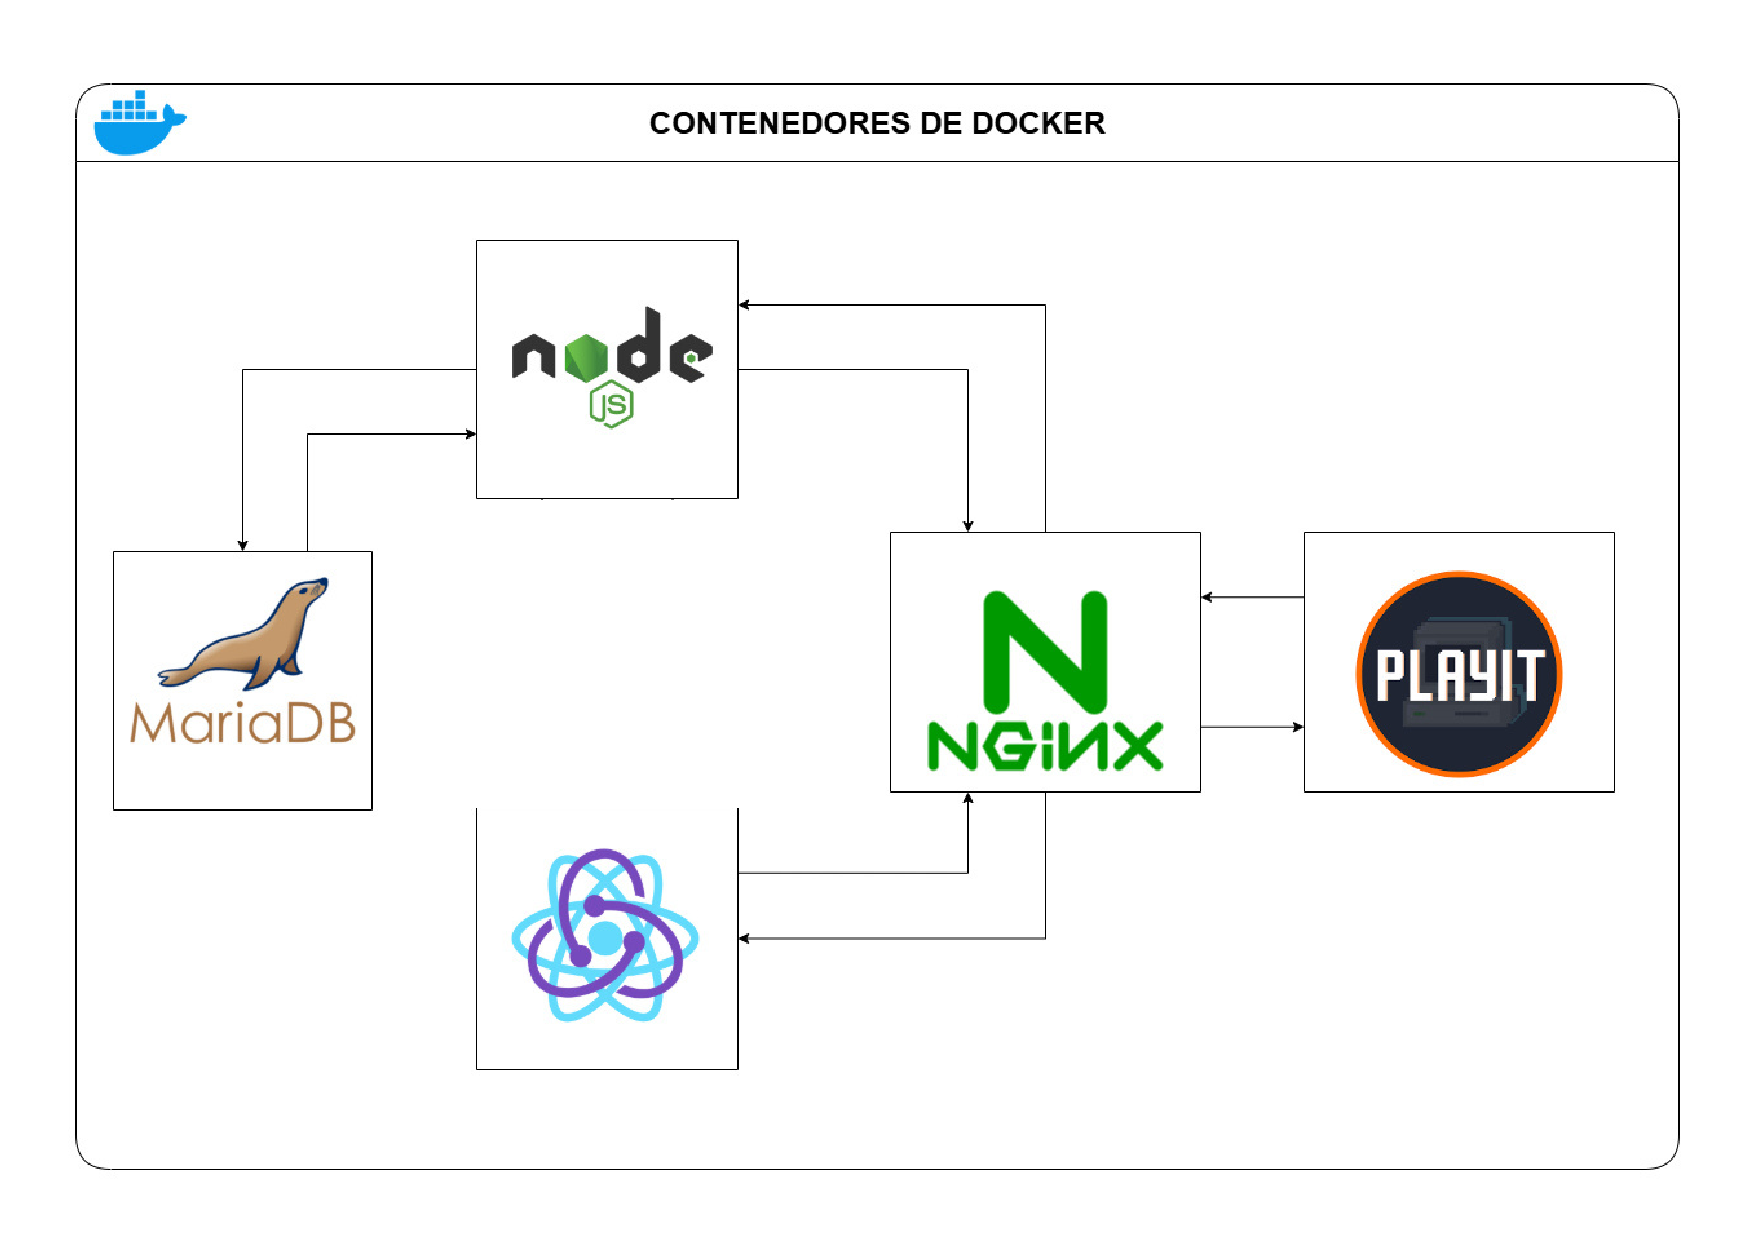
\includegraphics[width=1\textwidth]{Figs/Diagrama_contenedores.pdf}
	\label{fig:Diagrama-Docker}
	\\Fuente: Elaboración propia con base en la estructura de los contenedores usados.
\end{figure}

    \item \textbf{Material teórico en Moodle}
\begin{itemize}
	\item Se elaboraron recursos interactivos utilizando H5P dentro de Moodle.
	\item Los materiales incluyeron infografías sintetizadas, con la información esencial para el aprendizaje de los temas, permitiendo una mayor comprensión visual.
	\item La construcción de los contenidos se fundamentó en los textos de referencia de Montgomery y Walpole, autores reconocidos en estadística.
\end{itemize}

    \item \textbf{Graders en Google Colab}
\begin{itemize}
	\item Se desarrollaron notebooks en Google Colab con código en R.
	\item Estos graders permitieron calcular medidas de tendencia central y dispersión, así como generar representaciones gráficas (histogramas y diagramas de caja).
\end{itemize}

\item \textbf{Ejercicios calificables y lógica en el backend}
\begin{itemize}
	\item Se diseñaron tres ejercicios evaluables relacionados con los temas del sprint.
	\item Se implementó la lógica de corrección en el backend (Node.js) para procesar automáticamente las respuestas.
	\item El servidor de calificaciones registró y almacenó los resultados, garantizando un flujo de evaluación automatizado.
\end{itemize}
\end{enumerate}



\subsection{Sprint 2}

\subsubsection*{Objetivos del Scrum Master (docente)}
\begin{itemize}
	\item Definir los temas estadísticos a abordar: Teorema del Límite Central aplicado a la distribución t de Student y a la distribución F.
	\item Supervisar la ampliación de los recursos teóricos y prácticos, asegurando la coherencia pedagógica con el programa de la asignatura.
	\item Validar la correcta implementación de los graders relacionados con pruebas de hipótesis y comparación de varianzas.
	\item Orientar la mejora del \textit{frontend} para optimizar la visualización de las calificaciones y retroalimentaciones automáticas.
\end{itemize}

\subsubsection*{Cronograma del Sprint}
\begin{itemize}
	\item \textbf{Inicio del Sprint:} 16 de agosto de 2025 → Se definieron los temas estadísticos y se establecieron las prioridades técnicas.
	\item \textbf{Entrega de los practicantes:} 20 de agosto de 2025 → Se presentaron los nuevos materiales teóricos, graders funcionales y las primeras mejoras en la interfaz.
	\item \textbf{Revisión del Scrum Master:} 21 de agosto de 2025 → Se realizaron recomendaciones sobre la claridad conceptual de los contenidos y la usabilidad de la interfaz.
	\item \textbf{Liberación de recursos:} 22 de agosto de 2025 → Se publicaron en Moodle y Colab los materiales y graders validados para su uso en el entorno piloto.
\end{itemize}

\subsubsection*{Actividades realizadas por los practicantes}

\begin{enumerate}
	\item \textbf{Ampliación de contenidos teóricos}  
	\begin{itemize}
		\item Se elaboraron materiales interactivos en H5P centrados en el Teorema del Límite Central y su aplicación con distribuciones t de Student y F.
		\item Los contenidos incluyeron infografías, ejemplos resueltos y referencias bibliográficas, buscando facilitar la comprensión intuitiva de las distribuciones muestrales.
		\item Se enfatizó en la interpretación de regiones de rechazo, grados de libertad y supuestos estadísticos, para reforzar el razonamiento inferencial de los estudiantes.
	\end{itemize}
	
	\item \textbf{Graders de distribuciones t y F en Google Colab}  
	\begin{itemize}
		\item Se desarrollaron nuevos notebooks en Google Colab con código en R, enfocados en ejercicios prácticos sobre pruebas t y F.
		\item Los graders permitieron a los estudiantes realizar cálculos de valores críticos, regiones de rechazo y decisiones de hipótesis de forma automática.
		\item Se verificó su compatibilidad con el servidor de calificaciones y se implementaron pruebas para evitar errores de ejecución comunes.
	\end{itemize}
	
	\item \textbf{Ejercicios calificables y lógica en el backend}  
	\begin{itemize}
		\item Se diseñaron ejercicios evaluables sobre aplicaciones del Teorema del Límite Central, pruebas t y F, con distintos grados de dificultad.
		\item Se amplió la lógica en el backend para manejar retroalimentación más detallada, especificando en qué pasos se cometieron errores en la resolución.
		\item Se ajustaron los endpoints para almacenar no solo la nota final, sino también los comentarios generados automáticamente.
	\end{itemize}
	
	\item \textbf{Mejoras en el \textit{frontend} para visualización de calificaciones}  
	\begin{itemize}
		\item Se rediseñaron los componentes de interfaz relacionados con la visualización de notas y retroalimentaciones, mejorando la claridad y accesibilidad.
		\item Se incorporaron indicadores visuales que permiten a los estudiantes identificar rápidamente ejercicios aprobados, pendientes o con errores.
		\item Estas mejoras facilitaron la experiencia de usuario y contribuyeron a una retroalimentación más efectiva del proceso de aprendizaje.
	\end{itemize}
\end{enumerate}

\newpage

\chapter{Resultados}

Se presentan los resultados alcanzados en el diseño, implementación y validación del ambiente virtual de aprendizaje para el curso de Estadística II de la Escuela de Ingeniería de Sistemas e Informática de la UIS. Estos hallazgos evidencian el cumplimiento de los objetivos propuestos en la investigación, así como el impacto generado en los ámbitos pedagógico, tecnológico y estudiantil.

\section{Desarrollo tecnológico del ambiente virtual}

El proceso de implementación tecnológica del aula virtual de aprendizaje posibilitó la integración exitosa de diversas herramientas, garantizando su funcionamiento articulado y coherente.

Se utilizó como base la plataforma de gestión académica, en la cual se estructuraron los módulos temáticos del curso organizados por semanas como se evidencia en la Figura \ref{fig:Moodle}. En cada módulo se dispuso el contenido teórico a través de recursos interactivos que facilitaron al estudiante una visualización clara de los temas y de las fórmulas necesarias para su comprensión. Asimismo, se incorporaron recursos adicionales como guías de práctica como se muestra en el Anexo \ref{anexo:Guía Semana 8}, actividades y quices, con el fin de fortalecer el proceso de aprendizaje. 

\begin{figure}[ht]
	\centering
	\captionof{figure}{ \\ \vspace{0.5cm} Desarrollo tecnológico del ambiente virtual. \textbf{Estructura del curso de Moodle}.}
	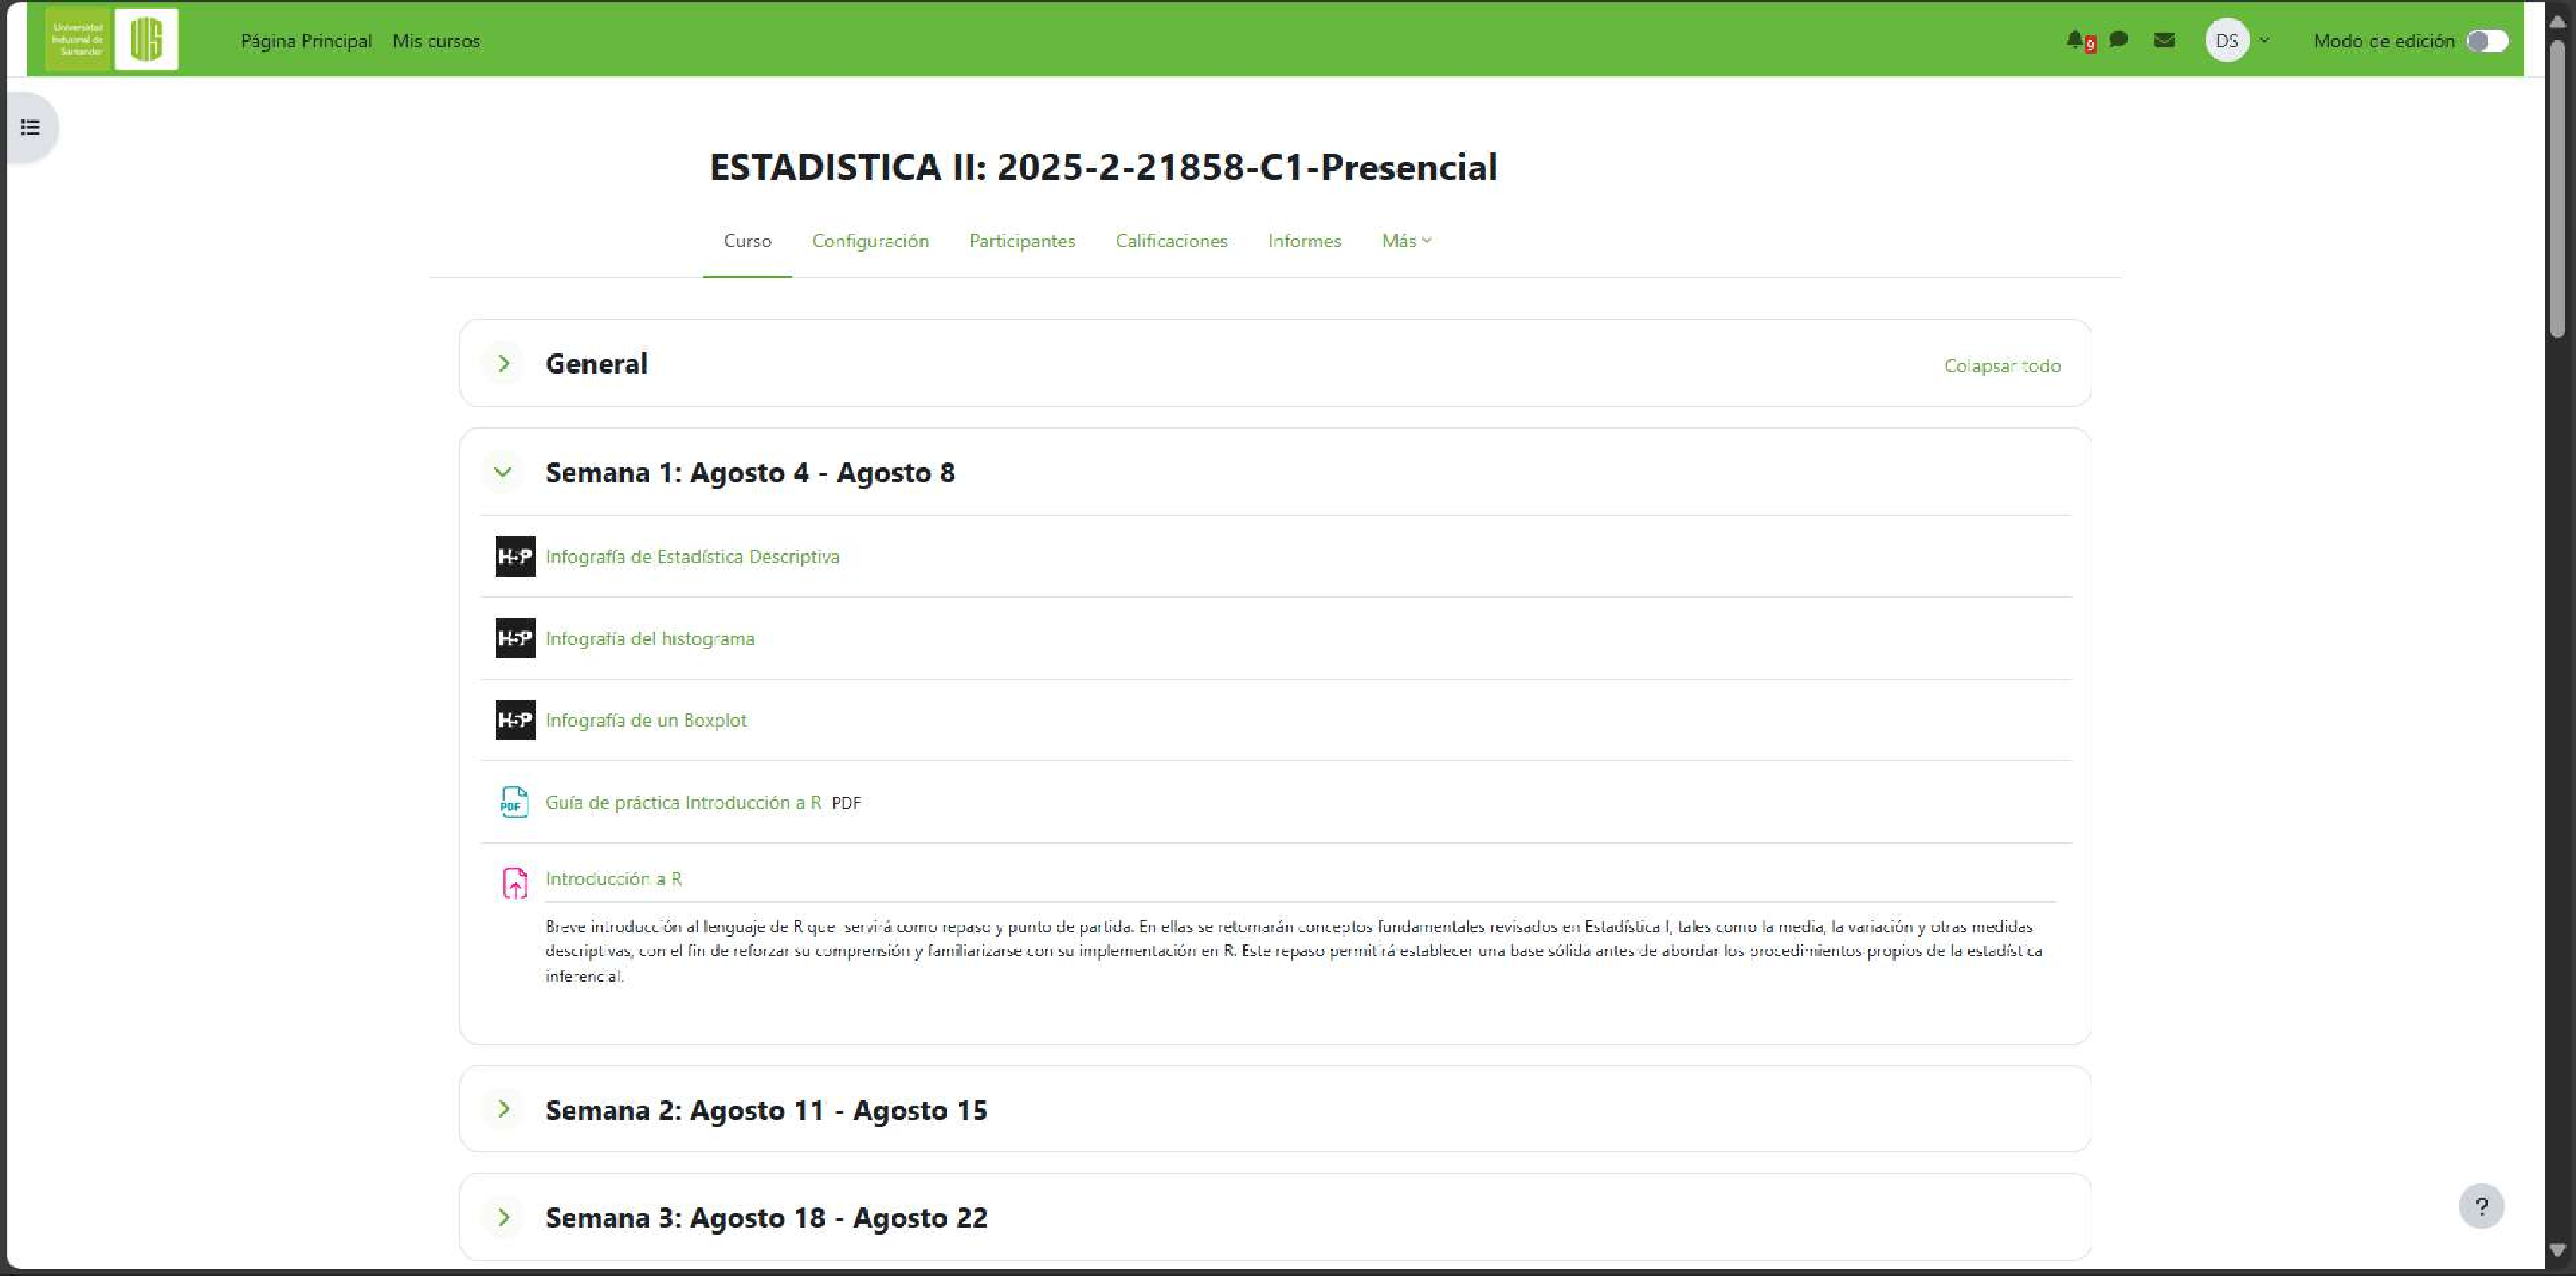
\includegraphics[width=1\textwidth]{Figs/Moodle.pdf}
	\label{fig:Moodle}
	\\Fuente: Pantallazo del curso en Moodle.
\end{figure}

\newpage

Vinculado a través de la plataforma, se utilizó el entorno virtual para realizar de ejercicios prácticos en R y Python, lo que permitió a los estudiantes aplicar de manera directa los conceptos teóricos aprendidos. Esta integración favoreció la resolución de los problemas estadísticos mediante programación, promoviendo el desarrollo de habilidades analíticas y computacionales, así como el aprendizaje activo y la comprensión profunda de los métodos estadísticos.

Los graders automáticos se integraron al aula virtual con el propósito de ofrecer a los estudiantes una retroalimentación inmediata de las prácticas. Gracias a esta herramienta, los estudiantes pudieron comprobar en tiempo real la validez de sus respuestas, identificar errores y comprender de manera más clara los pasos necesarios para llegar a la solución correcta. Así, además de agilizar la evaluación, se promovió una participación más autónoma y activa; los estudiantes tenían la oportunidad de corregir desde su propia experiencia.

Se implementó el plugin \textit{Safe Exam Browser (SEB)} en los quices del curso. Esta herramienta permite bloquear el acceso a otras aplicaciones, navegadores o páginas web mientras los estudiantes realizan los ejercicios, asegurando que cada cuestionario se responda de manera individual y bajo condiciones controladas. Aportando ventajas significativas como:

\begin{itemize}
    \item \textbf{Prevenir distracciones y accesos no autorizados:} los estudiantes no podían navegar fuera del entorno de evaluación, lo que permitió mantener su atención centrada en los ejercicios.
    \item \textbf{Fortalecer la confiabilidad de los resultados:} los datos reflejaron únicamente el desempeño individual de cada estudiante, ofreciendo información más precisa sobre su aprendizaje.
\end{itemize}

Gracias a estas características, SEB no solo reforzó la seguridad de los quices, sino que también contribuyó a crear un entorno más confiable y justo para los estudiantes, promoviendo una experiencia de aprendizaje más seria y comprometida.

\section{Infraestructura tecnológica implementada}

La infraestructura tecnológica diseñada para soportar el ambiente virtual de aprendizaje se estructuró bajo un modelo basado en contenedores \textit{Docker}, lo que permitió separar los distintos servicios y garantizar su portabilidad y escalabilidad. El despliegue general se gestionó mediante el archivo \texttt{docker-compose.yml} en un computador personal de 12 GB de ram en un sistema operativo UBUNTU de Linux, que coordinó la ejecución simultánea de cada servicio como se muestra en la Figura \ref{fig:AVA}. La organización de los servicios se estructuró de la siguiente manera:

\begin{figure}[ht]
	\centering
	\captionof{figure}{ \\ \vspace{0.5cm} Infraestructura tecnológica implementada. \textbf{Arquitectura tecnológica del Ambiente Virtual de aprendizaje}.}
	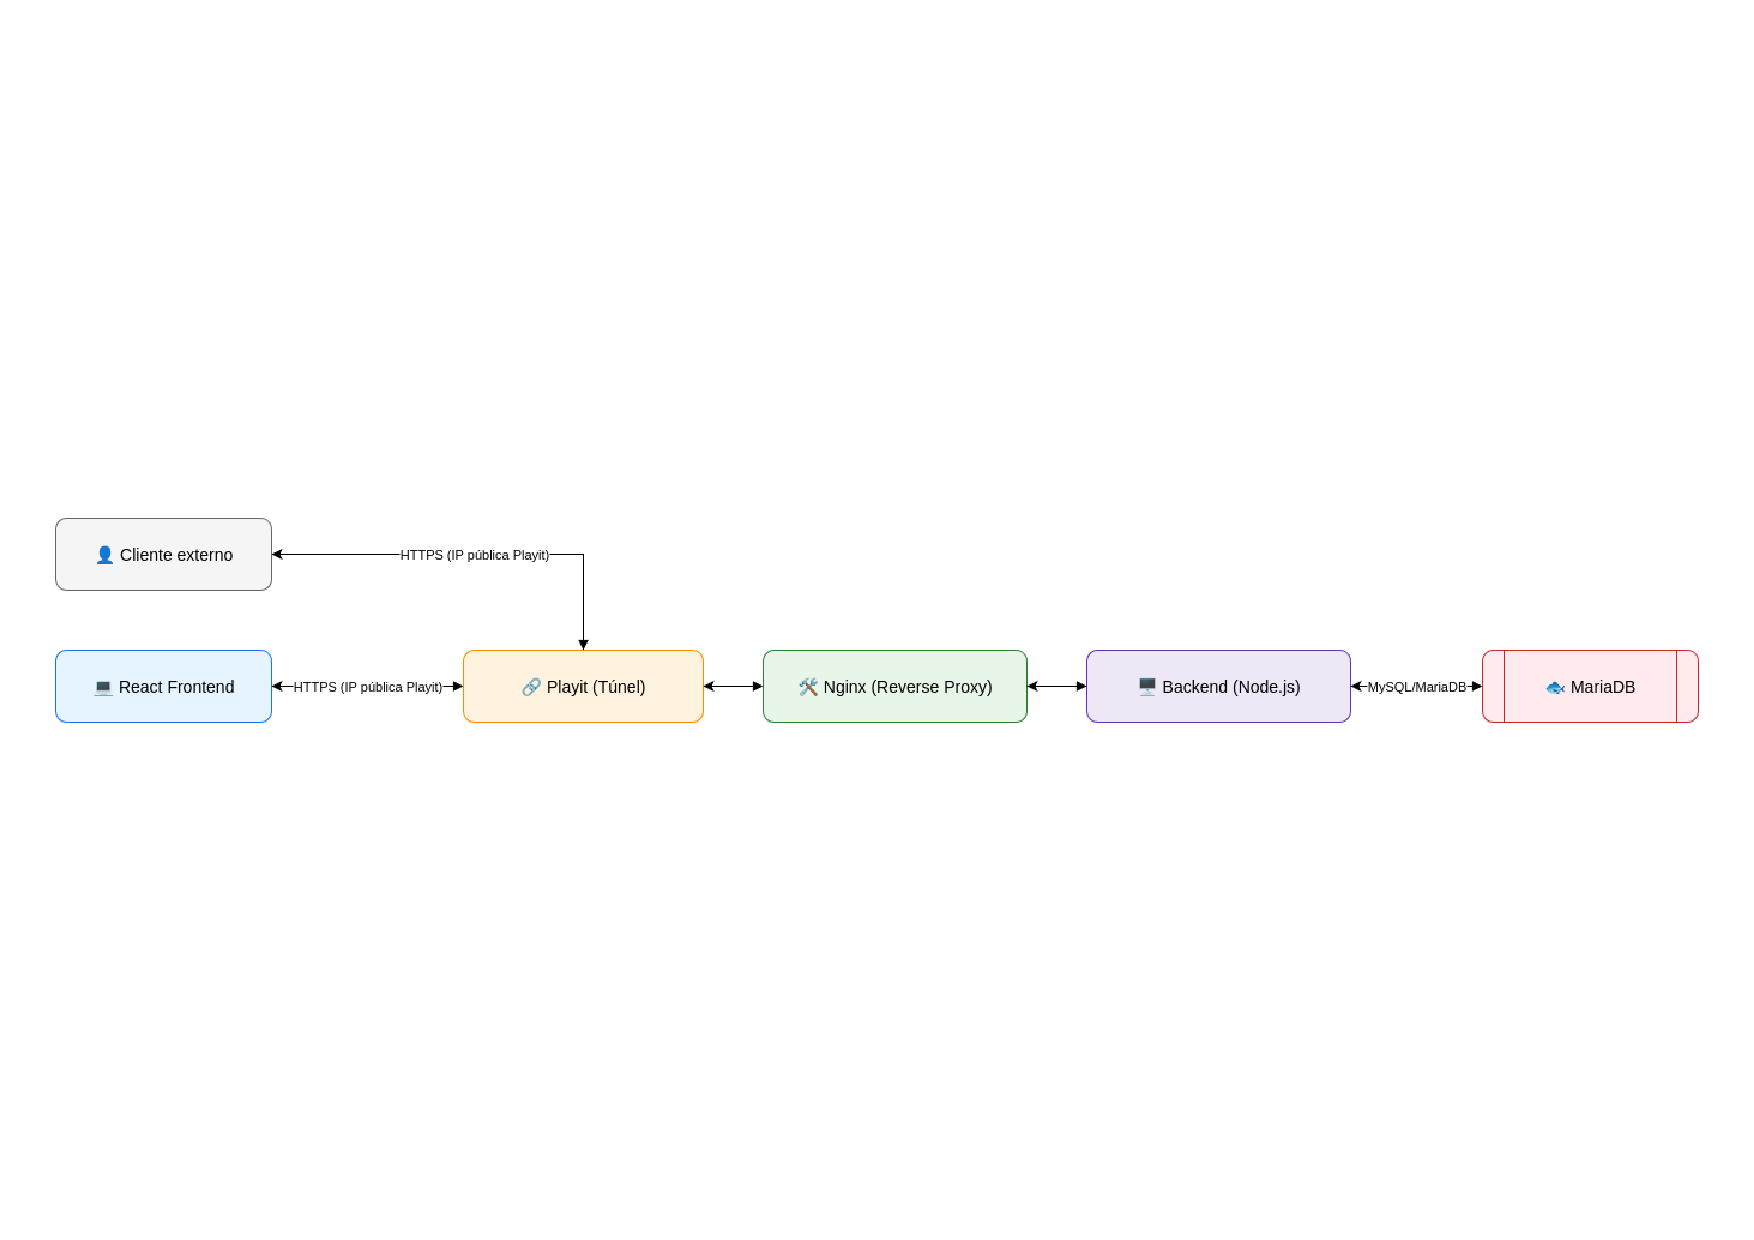
\includegraphics[width=0.7\textwidth]{Figs/Arquitectura_AVA.pdf}
	\label{fig:AVA}
	\\Fuente: Elaboración propia segun el árbol de estructura de servicios.
\end{figure}

\subsection{Backend}
\begin{itemize}
    \item Contiene la lógica principal del sistema desarrollada en \textit{Node.js}.
    \item El archivo \texttt{server.js} y la carpeta \texttt{src/app.js} gestionan la configuración base del servidor.
    \item En la carpeta \texttt{controllers} se desarrollaron los controladores para las diferentes prácticas (\texttt{prac1.controller.js}, \texttt{prac2.controller.js}, etc.), el manejo de estudiantes y la comunicación con la interfaz de frontend.
    \item En \texttt{routes} se definieron las rutas para estudiantes, cuestionarios y la interacción con el frontend.
    \item La carpeta \texttt{config/db.js} centralizó la conexión con la base de datos.
\end{itemize}

\subsection{Frontend}
\begin{itemize}
    \item Implementado con \textit{React}, contenía la interfaz con la que interactuaron los practicantes y el docente.
    \item En la carpeta \texttt{components} se construyeron elementos como \texttt{Grupos.js}, \texttt{Semanas.js} y \texttt{DetalleEstudiante.js}, que organizaron la presentación de la información académica.
    \item Los estilos \texttt{CSS} asociados (\texttt{Grupos.css}, \texttt{Semanas.css}, \texttt{DetalleEstudiantes.css}) se diseñaron para lograr una visualización limpia y funcional.
    \item El despliegue del \textit{frontend} se gestionó mediante un \texttt{Dockerfile}, asegurando que la interfaz se integrara de manera coherente al ecosistema.
\end{itemize}

\subsection{Base de Datos}
\begin{itemize}
    \item Se utilizó \textit{MariaDB} como sistema gestor, con inicialización automática mediante el archivo \texttt{init.sql}.
    \item La persistencia se garantizó con el volumen \texttt{mariadb\_data}.
\end{itemize}

\subsection{Nginx}
\begin{itemize}
    \item Funcionó como servidor web y proxy inverso, controlando el acceso externo al sistema.
    \item El archivo \texttt{nginx.conf} definió las reglas de enrutamiento.
    \item La carpeta \texttt{certs} almacenó los certificados de seguridad (\texttt{fullchain.pem} y \texttt{privkey.pem}), junto con la configuración del certificado SAN (\texttt{san.cnf}) para habilitar la navegación segura mediante \texttt{HTTPS}.
    \item Los registros de acceso y errores (\texttt{logs/access.log}, \texttt{logs/error.log}) facilitaron la monitorización del sistema.
\end{itemize}

\subsection{Playit.gg}
\begin{itemize}
    \item Durante la implementación de los grupos piloto, se utilizó este servicio para establecer túneles seguros y exponer temporalmente los servicios.
    \item Esto garantizó la accesibilidad sin necesidad de un despliegue en un servidor hosting.
\end{itemize}

\section{Recursos interactivos}

Además de la infraestructura tecnológica y los servicios de programación, el ambiente virtual de aprendizaje integró herramientas digitales especialmente orientadas a enriquecer la experiencia pedagógica de los estudiantes mediante contenidos dinámicos e interactivos.

En este contexto, se hizo uso de \textit{Genially} y \textit{H5P}, plataformas que permitieron diseñar materiales innovadores y atractivos, con el objetivo de facilitar la comprensión de los conceptos teóricos y metodológicos de \textit{Estadística II}. Genially se destinó principalmente a la elaboración de infografías y presentaciones interactivas como se muestran en las Figuras \ref{fig:Pgenially} y \ref{fig:Igenially}, que transformaron información compleja en representaciones visuales claras y accesibles. Estos recursos, una vez integrados en \textit{Moodle}, se convirtieron en un apoyo valioso para los distintos módulos del curso, ya que brindaron a los estudiantes la posibilidad de interactuar con los contenidos y explorar los temas de manera autónoma.

\begin{figure}[ht]
	\centering
	\captionof{figure}{ \\ \vspace{0.5cm} Recursos interactivos. \textbf{Presentación en Genially sobre Intervalos de confianza}.}
	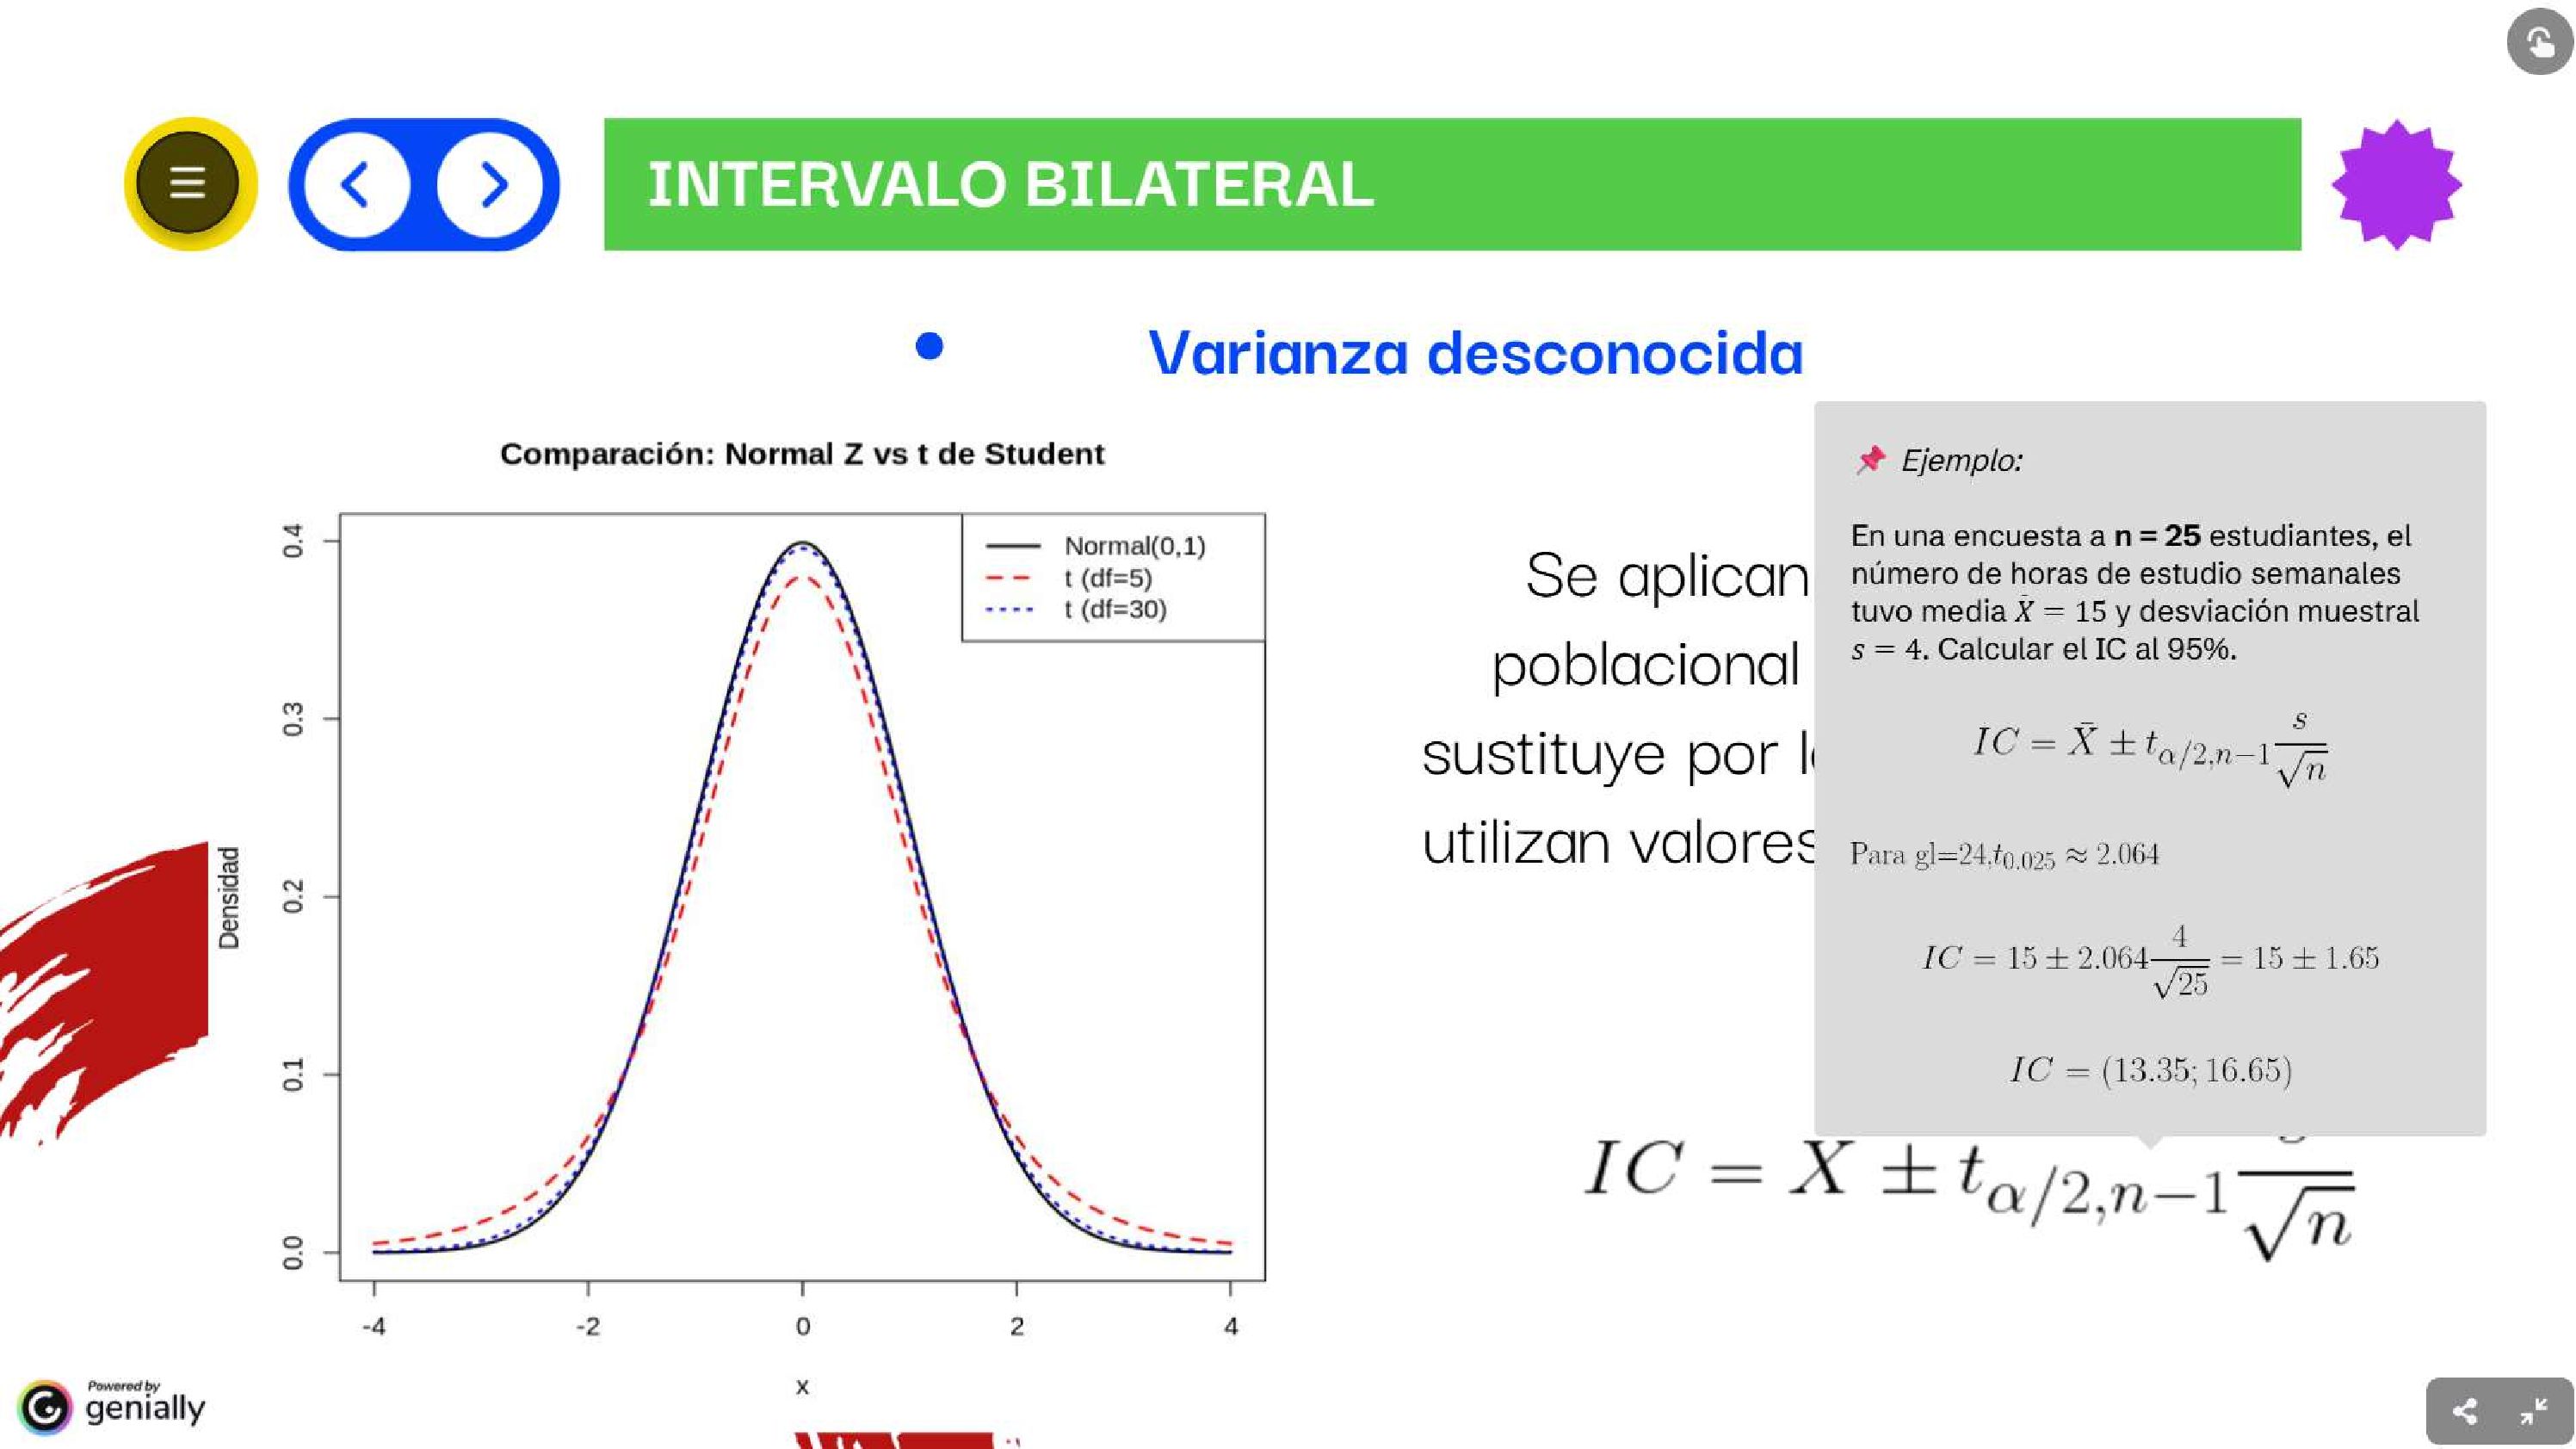
\includegraphics[width=1\textwidth]{Figs/Presentacion_Genially.pdf}
	\label{fig:Pgenially}
	\\Fuente: Pantallazo de una presentación en Genially.
\end{figure}

\begin{figure}[ht]
	\centering
	\captionof{figure}{ \\ \vspace{0.5cm} Recursos interactivos. \textbf{Infografía en Genially sobre Bootstrap}.}
	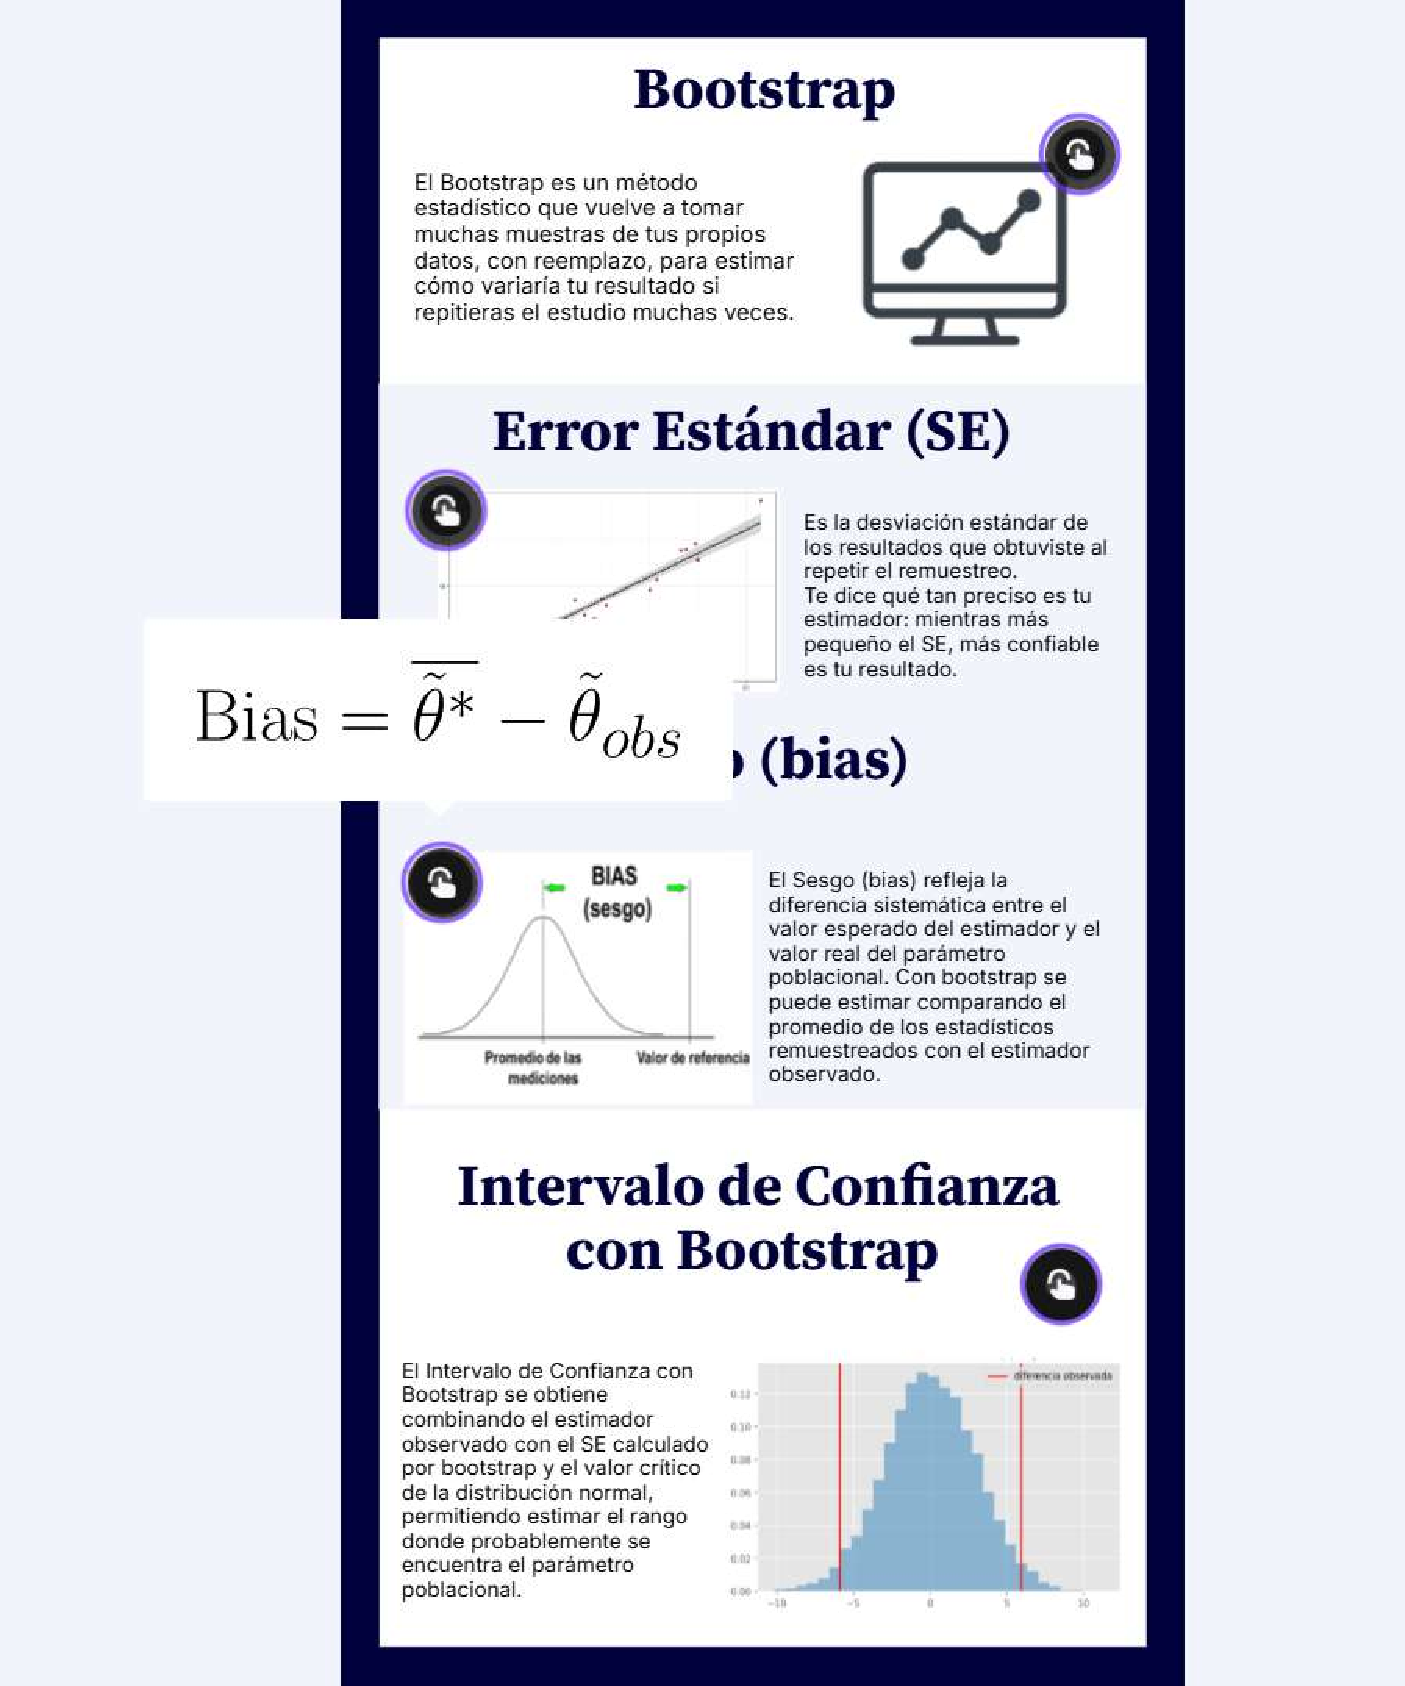
\includegraphics[width=0.6\textwidth]{Figs/Infografia_Genially.pdf}
	\label{fig:Igenially}
	\\Fuente: Pantallazo de una infografía en Genially.
\end{figure}

Por su parte, \textit{H5P}, que puede implementarse de forma nativa en \textit{Moodle}, se utilizó para generar infografías y actividades en las primeras clases como se muestra en la Figura \ref{fig:H5P}, contribuyendo a un aprendizaje más activo desde el inicio del curso. En el caso de \textit{Genially}, debido a que no se integra directamente en la plataforma, se recurrió al uso de \textit{iframes} embebidos para incorporar materiales sobre temas complejos, como el Teorema del Límite Central, en los cuales se añadieron diagramas interactivos y simulaciones.

\begin{figure}[ht]
	\centering
	\captionof{figure}{ \\ \vspace{0.5cm} Recursos interactivos. \textbf{Infografía en H5P sobre Estadística descriptiva}.}
	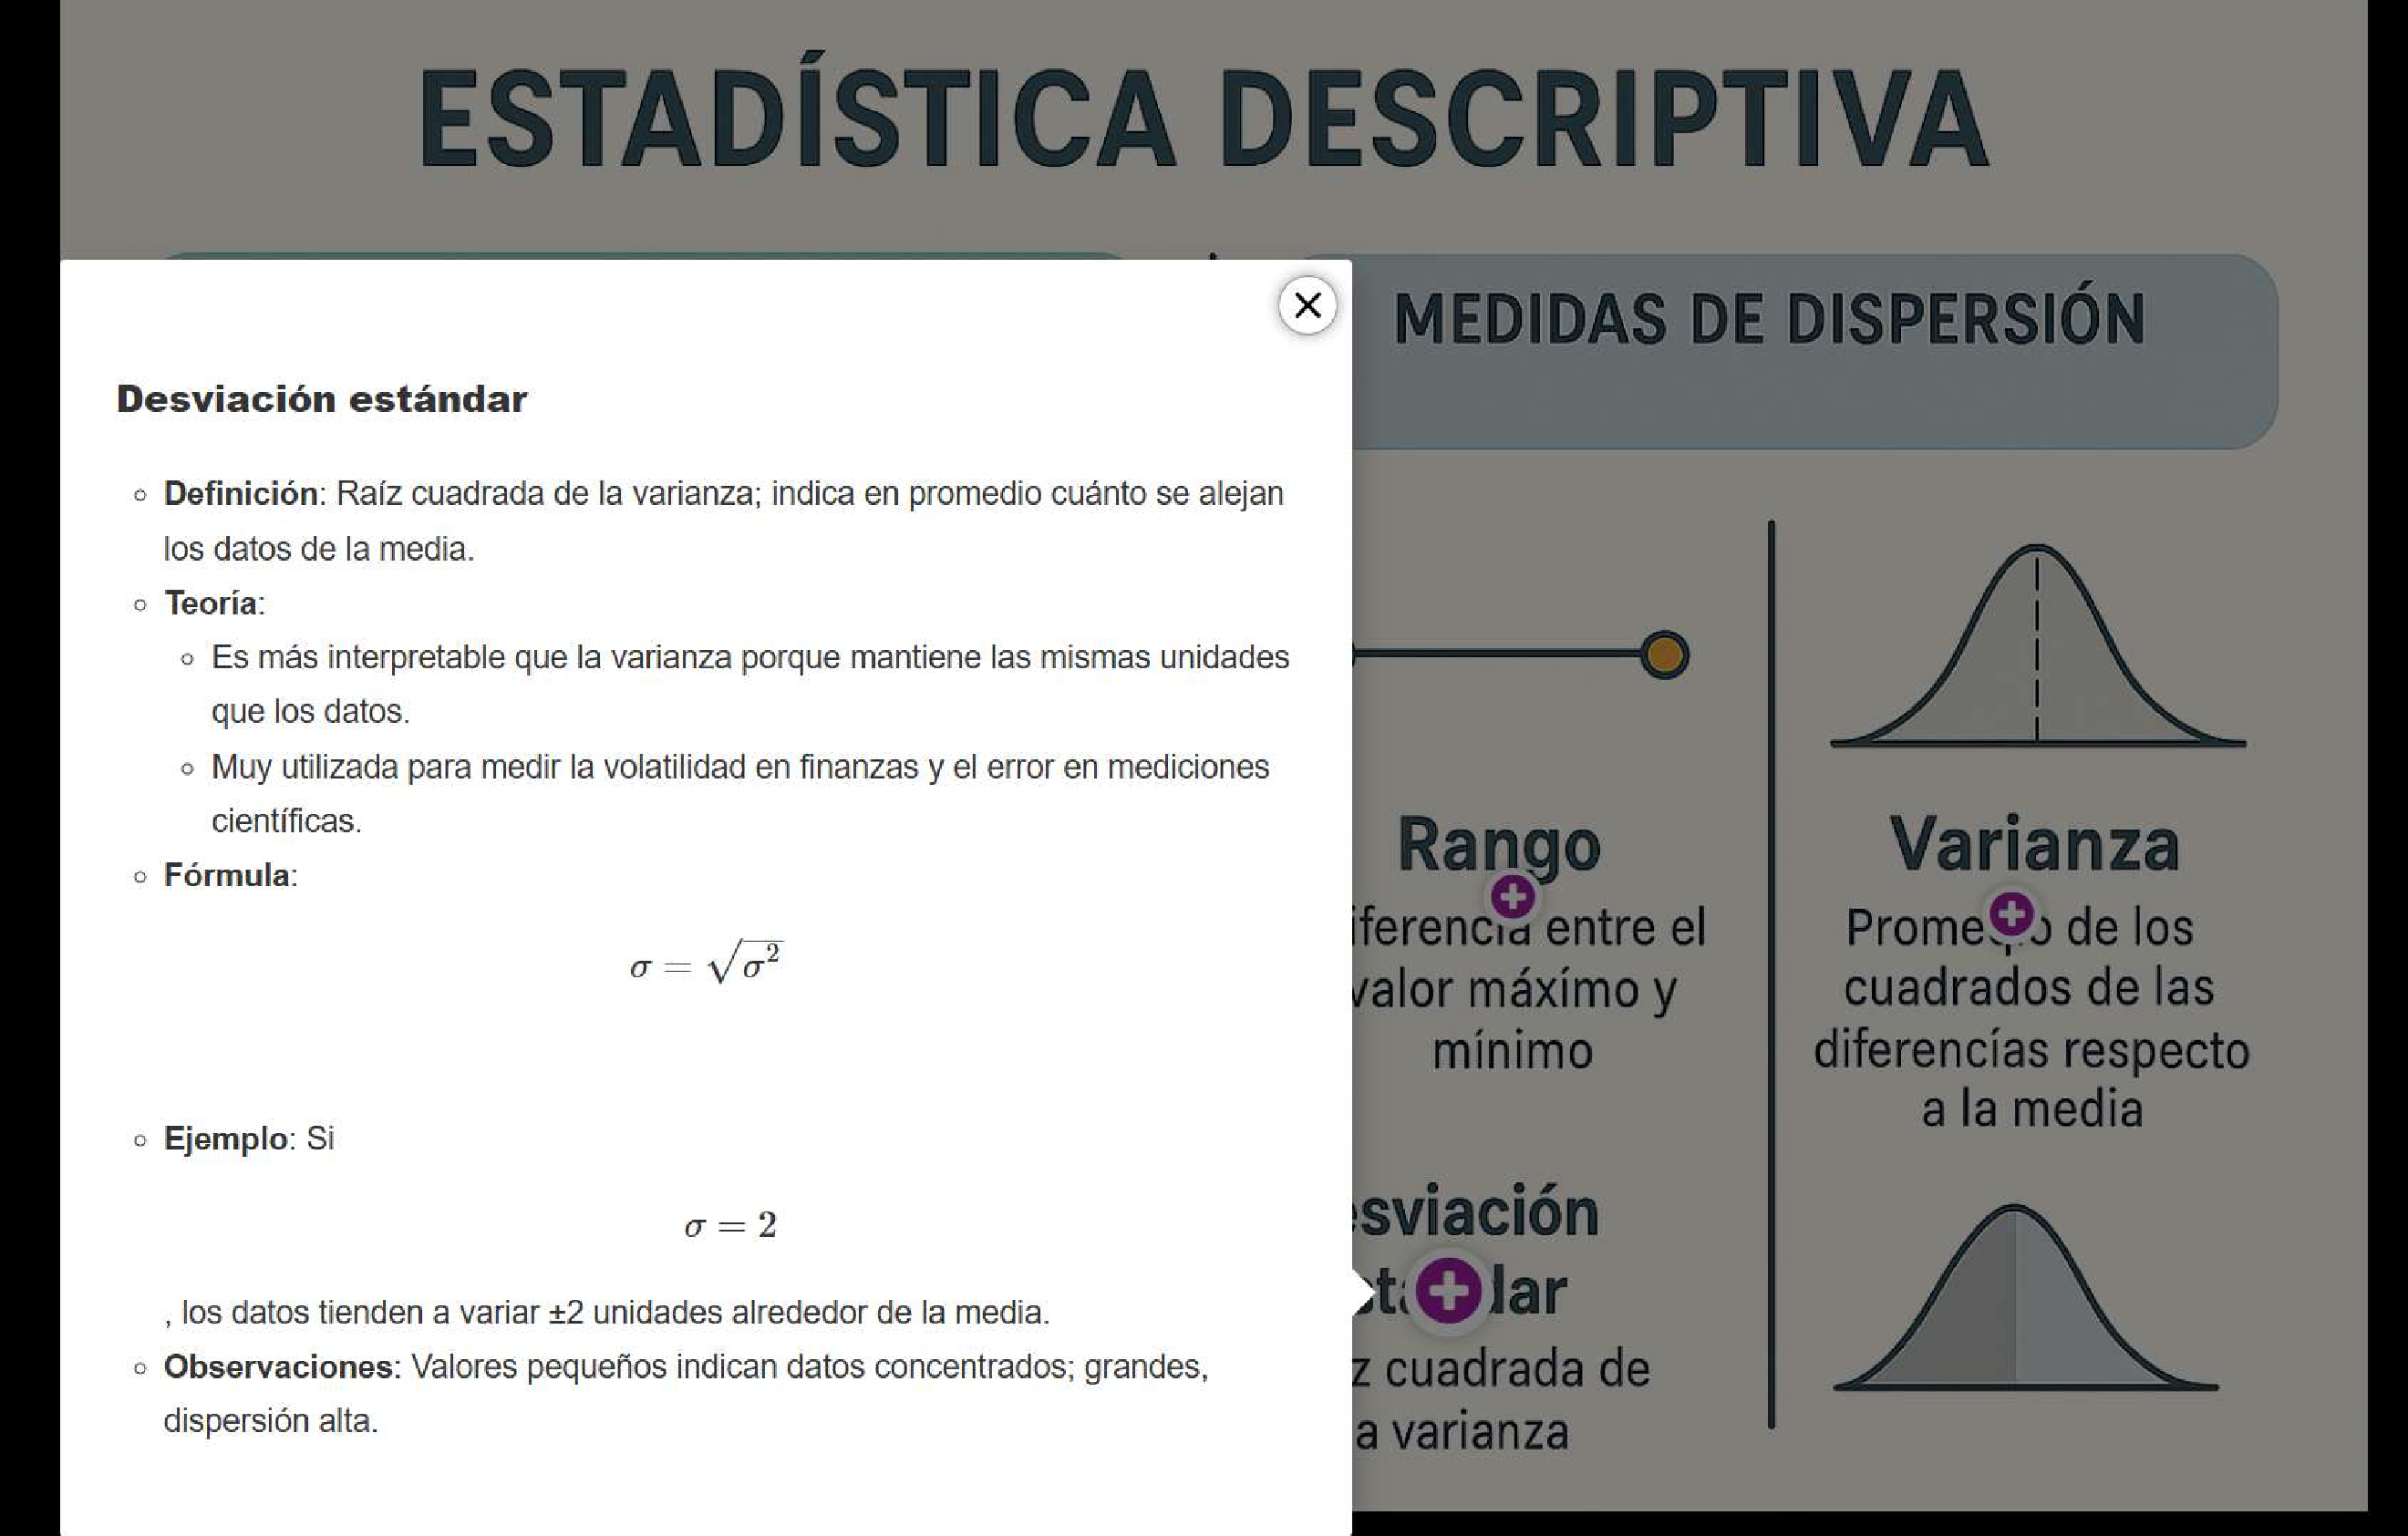
\includegraphics[width=1\textwidth]{Figs/Infografia_H5P.pdf}
	\label{fig:H5P}
	\\Fuente: Pantallazo de una infografía en H5P.
\end{figure}

Este proceso contó con el acompañamiento del profesor Carlos Mantilla, quien no solo orientó en la correcta implementación de los recursos embebidos, sino que también brindó recomendaciones sobre la manera más efectiva de llevar los temas dentro de \textit{Moodle}.

\section{Experiencia de los Estudiantes}

Un componente central en la evaluación de resultados fue la percepción de los estudiantes frente al uso del entorno y las herramientas tecnológicas. Para ello, se aplicó una encuesta a los dos cursos participantes, con el fin de indagar tanto en la experiencia técnica como en el impacto académico.

\newpage

\chapter{Conclusiones y trabajo a futuro}

\newpage
% ------------------------------------------------------------------------
% Bibliografía
% ------------------------------------------------------------------------

%\addcontentsline{toc}{chapter}{Referencias Bibliográficas}\newpage
%\bibliographystyle{apalike}
%\bibliography{biblio}
\addcontentsline{toc}{chapter}{Referencias Bibliográficas}

\printbibliography

\nocite{poniszewska-maranda, burns-kubernetes, torres-bosch-microservicios, armstrong2015,kubevirtio, docker2023, kubelet-doc, namespace-article}
% ------------------------------------------------------------------------
% Anexos
\newpage

\appendix

% --- Solo una entrada en la TOC ---
\chapter*{Anexos}
\addcontentsline{toc}{chapter}{Anexos}

% --- Definir numeración en números ---
\renewcommand{\thechapter}{\arabic{chapter}}

% --- Anexo 1 ---
\refstepcounter{chapter}
\chapter*{Anexo \thechapter: Actas de reunión}
\label{anexo:actas}

\section*{Acta de reunión inicial - 02 de abril de 2025}
\label{anexo:acta-abril-2025}

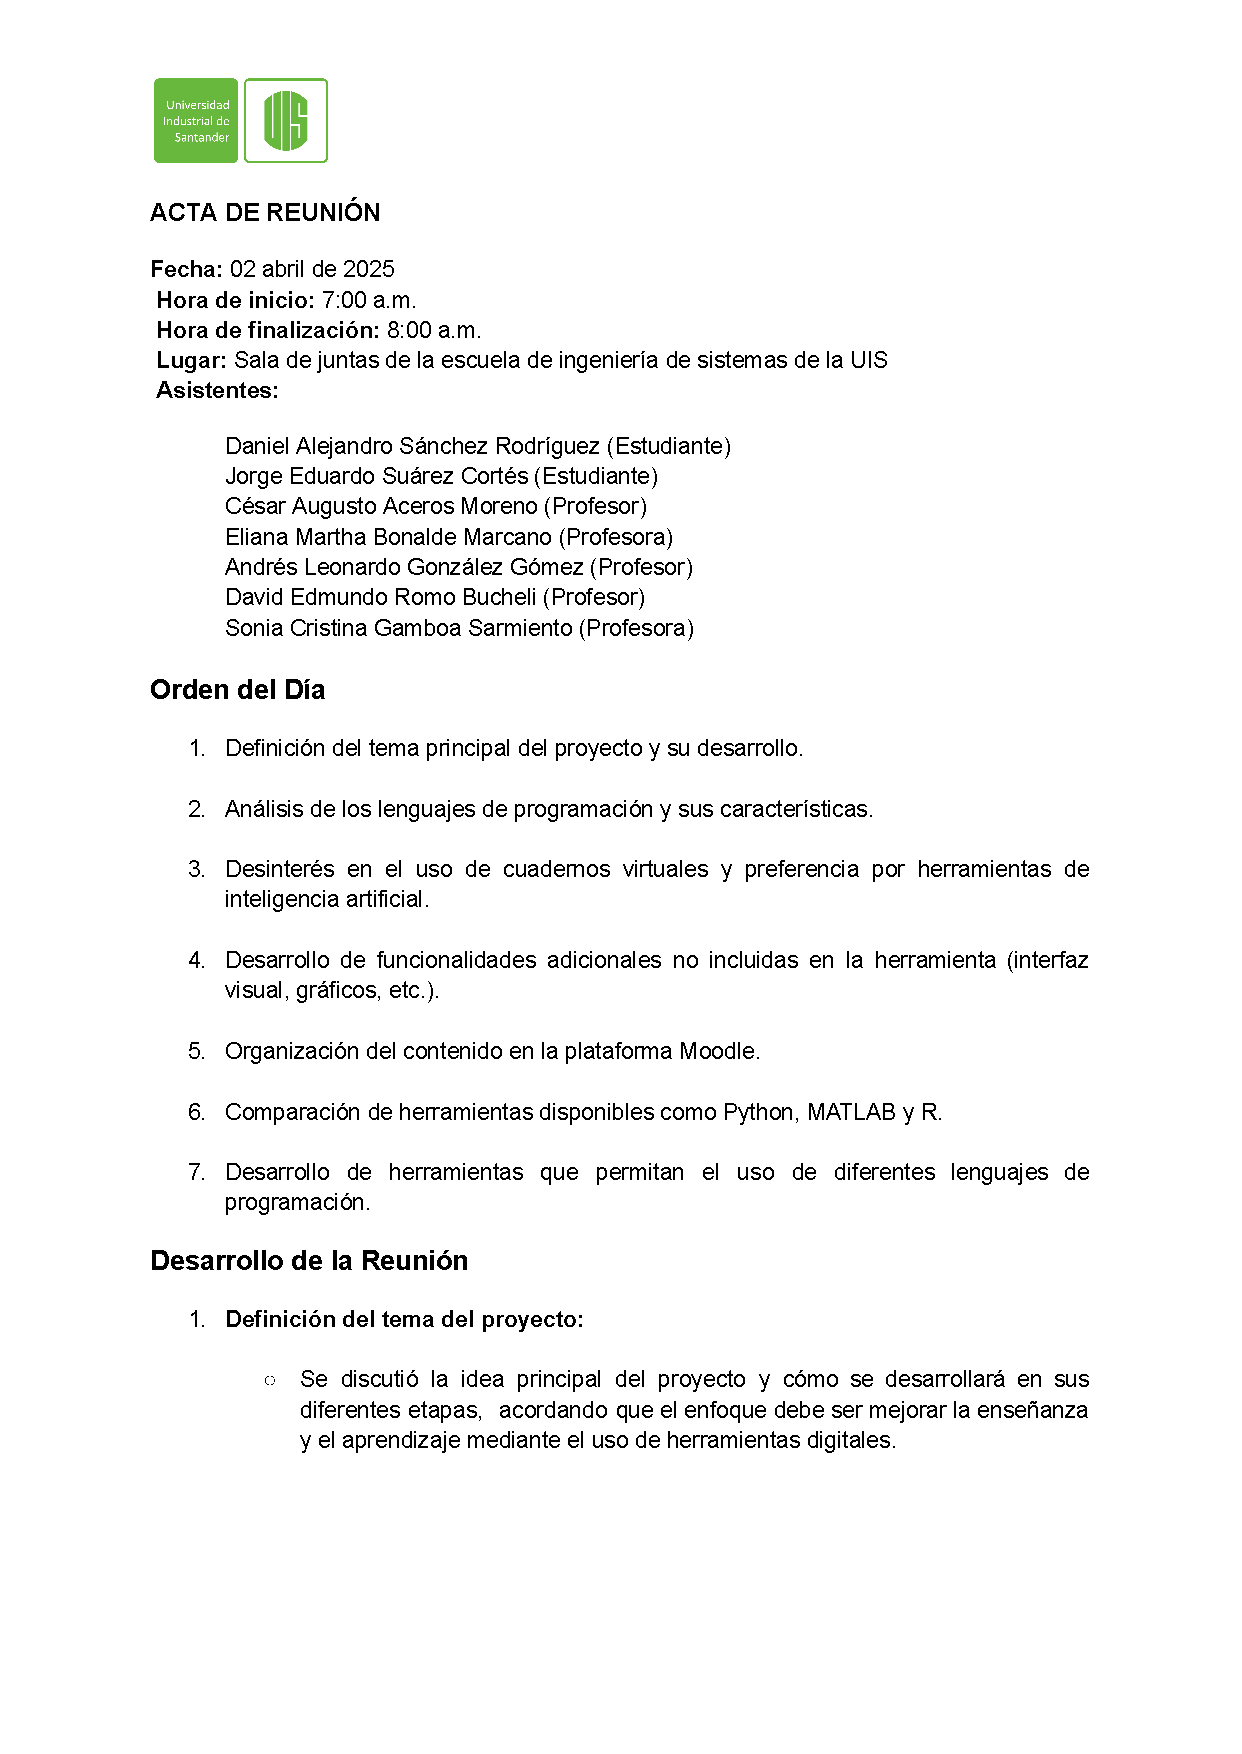
\includepdf[pages=-, scale=0.9, pagecommand={\thispagestyle{plain}}]{Anexos/Acta 02 abril de 2025.pdf}

\refstepcounter{chapter}
\chapter*{Anexo \thechapter: Guías de prácticas}
\label{anexo:Guía Semana 8}

\section*{Guía de práctica de la semana 8}
\label{anexo:Guía-Semana-8}

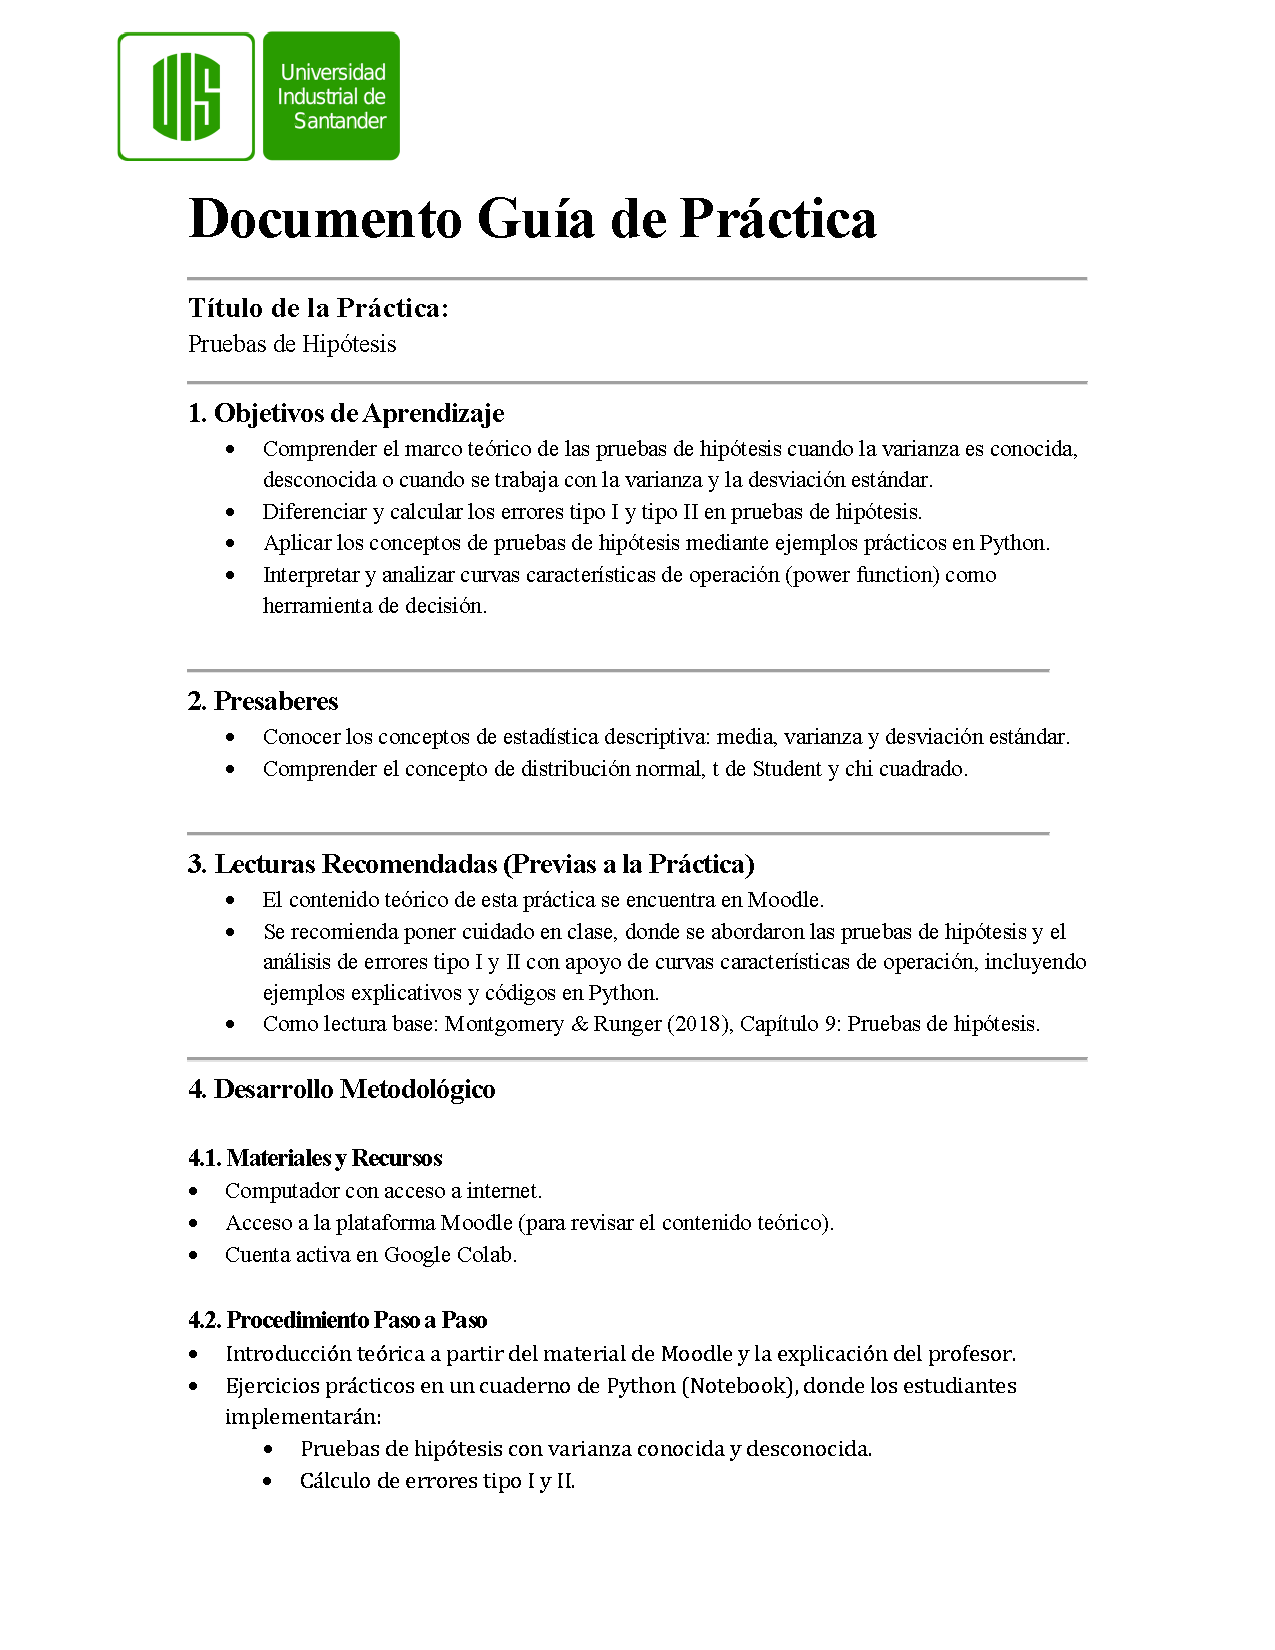
\includepdf[pages=-, scale=0.9, pagecommand={\thispagestyle{plain}}]{Anexos/G.pdf}
% ------------------------------------------------------------------------

% ------------------------------------------------------------------------
\end{document}                                          % Fin de documento
% ------------------------------------------------------------------------ 
